<<<<<<< HEAD
\begin{name}
	{\tenchude}
	{ĐỀ TT LẦN 2 - SỞ NINH BÌNH}
	{LỚP TOÁN THẦY PHÁT}
	{{Alle sagten, das geht nicht. \\Dann kam Einer, der wusste das nicht, und hat’s einfach gemacht.}}
\end{name}
\caulc
\Opensolutionfile{ans}[ans/ans\currfilebase]
%Câu 1
\begin{ex}%[2D1B3-1]%[Dự án đề TT Toán NH25-26 Đợt 3- Nguyễn Thành Tiến]%[TT-SGD-Ninh Bình - Ninh BÌnh]%[GVPB: Phạm Văn Long]
	\immini[thm]{
		Cho hàm số $y=f(x)$ liên tục trên đoạn $[-2;3]$ và có đồ thị trong hình bên. Giá trị lớn nhất của hàm số $y=f(x)$ trên đoạn $[-2 ; 3]$ bằng bao nhiêu?
		\choice
		{$1$}
		{$3$}
		{$-3$}
		{\True $2$}
	}{
		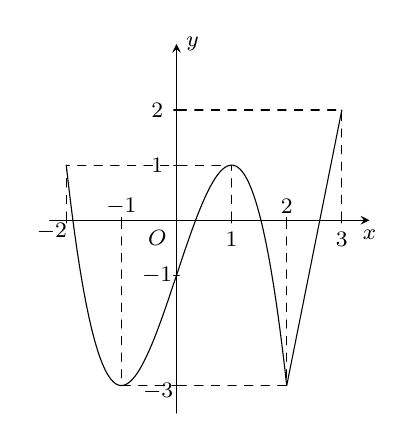
\begin{tikzpicture}[line join = round, line cap = round,font=\footnotesize,>=stealth,scale=.7] 
			\draw[->](-2.3,0)--(3.5,0)node[below]{$x$};
			\draw[->](0,-3.5)--(0,3.2)node[right]{$y$};
			\draw (0,0)node[below left]{$O$};
			\def\a{-1};
			\def\b{0};
			\def\c{3};
			\def\d{-1};
			\def\f(#1){\a*(#1)^3+\b*(#1)^2+\c*(#1)+\d};
			\draw[domain=-2:2,samples=100,smooth]plot(\x,{\f(\x)});
			\draw[dashed] (-2,0)--(-2,1)--(0,1) (1,0)--(1,1)--(0,1) (2,0)--(2,-3)--(0,-3) (-1,0)--(-1,-3)--(0,-3) (3,0)--(3,2)--(0,2);
			\draw (2,-3)--(3,2);
			\foreach \x/\g in {-2/-150,-1/90,1/-90,2/90,3/-90}\draw (\x,.05)--(\x,-.05)+(\g:.3)node{$\x$};
			\foreach \x/\g in {-3/-160,-1/180,1/180,2/180}\draw (.05,\x)--(-0.05,\x)+(\g:.3)node{$\x$};
		\end{tikzpicture}
	}
	\loigiai{
		Từ đồ thị hàm số, suy ra $\max\limits_{\left[-2;3\right]} f(x)=f(3)=2$
	}
\end{ex}

\begin{ex}%[2D1Y1-2]%[Dự án đề TT Toán NH25-26 Đợt 3- Nguyễn Thành Tiến]%[TT-SGD-Ninh Bình - Ninh BÌnh]%[GVPB: Phạm Văn Long]
	Cho hàm số $y=f(x)$ có bảng biến thiên như sau:
	\begin{center}
		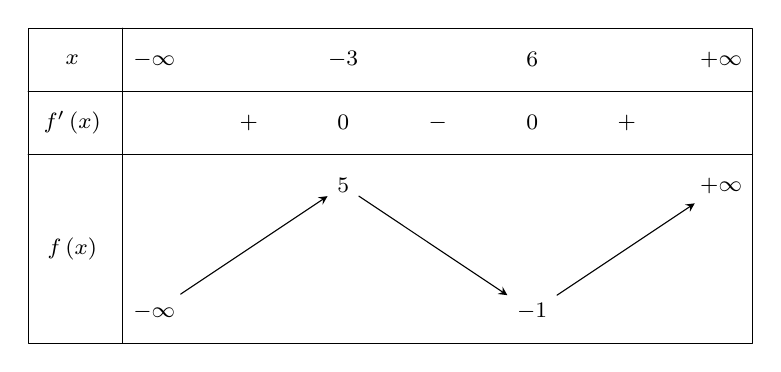
\begin{tikzpicture}[line join = round, line cap = round,font=\footnotesize,>=stealth,scale=.8]
			\foreach \x/\g in{-.3/x,1/-\infty,4/-3,7/6,10/+\infty}\path(\x,0)node{$\g$};
			\foreach \x/\g in {-.3/f'\left(x\right),2.5/+,4/0,5.5/-,7/0,8.5/+}\path(\x,-1)node{$\g$};
			\foreach \x/\y/\g in {-.3/-3/f\left(x\right),1/-4/-\infty,4/-2/5,7/-4/-1,10/-2/+\infty}\path(\x,\y)node(\x){$\g$};
			\foreach \x/\y in {1/4,4/7,7/10}\draw[-stealth] (\x)--(\y);
			\draw
			(-1,.5) rectangle (10.5,-4.5)
			(-1,-.5)--(10.5,-.5)
			(-1,-1.5)--(10.5,-1.5)
			(.5,.5)--(.5,-4.5);
		\end{tikzpicture}
	\end{center}
	Hàm số đã cho đồng biến trên khoảng nào sau đây?
	\choice
	 {$(-3;6)$}
	{\True $(6;+\infty)$}
	{$(-1;+\infty)$}
	{$(-\infty;5)$}
	\loigiai{
		Từ bảng biến thiên suy ra hàm số đồng biến trên các khoảng $(-\infty;-3)$ và $(6;+\infty)$. 
	}
\end{ex}

\begin{ex}%[2D3B2-1]%[Dự án đề TT Toán NH25-26 Đợt 3- Nguyễn Thành Tiến]%[TT-SGD-Ninh Bình - Ninh BÌnh]%[GVPB: Phạm Văn Long]
	Cho hàm số bậc hai $f(x)$. Biết đồ thị hàm số $y=f(x)$ cắt đường thẳng $y=9 x+8$ tại hai điểm $A$, $B$ phân biệt có hoành độ lần lượt là $x_A=-1$, $x_B=4$. Tính $I=\displaystyle\int\limits_{-1}^4 f'(x) \mathrm{\,d}x$.
	\choice
	{$I=43$}
	{$I=30$}
	{\True $I=45$}
	{$I=5$}
	 \loigiai{
		Theo giả thiết, ta suy ra $f(4)=y(4)=44$ và $f(-1)=y(-1)=-1$.\\
		Do đó
		\begin{eqnarray*}
			\displaystyle\int\limits_{-1}^4 f'(x) \mathrm{\,d}x=f(x)\Big|_{-1}^{4}=f(4)-f(-1)=44-(-1)=45.
		\end{eqnarray*}
	} 
\end{ex}

\begin{ex}%[2D3Y2-1]%[Dự án đề TT Toán NH25-26 Đợt 3- Nguyễn Thành Tiến]%[TT-SGD-Ninh Bình - Ninh BÌnh]%[GVPB: Phạm Văn Long]
	Nếu $\displaystyle\int\limits_0^1 f(x) \mathrm{\,d}x=2$ và $\displaystyle\int\limits_1^3 f(x) \mathrm{\,d}x=8$ thì $\displaystyle\int\limits_0^3 f(x) \mathrm{\,d}x$ bằng
	\choice
	{$16$}
	{$4$}
	{\True $10$}
	{$6$}
	\loigiai{
		Ta có
		\begin{eqnarray*}
			\displaystyle\int\limits_0^3 f(x) \mathrm{\,d}x&=&\displaystyle\int\limits_0^1 f(x) \mathrm{\,d}x+\displaystyle\int\limits_1^3 f(x) \mathrm{\,d}x\\
			&=&2+8=10.
		\end{eqnarray*}
	}
\end{ex}

\begin{ex}%[2H3B1-1]%[Dự án đề TT Toán NH25-26 Đợt 3- Nguyễn Thành Tiến]%[TT-SGD-Ninh Bình - Ninh BÌnh]%[GVPB: Phạm Văn Long]
	\immini[thm]{
		Cho hình lập phương $ABCD.A'B'C'D'$ (xem hình bên). Vectơ $\overrightarrow{AB}$ bằng vectơ nào sau đây?
		\choice
		{$\overrightarrow{CD}$}
		{$\overrightarrow{BC}$}
		{$\overrightarrow{AA'}$}
		{\True $\overrightarrow{A'B'}$}
	}{
		\begin{tikzpicture}[line join = round, line cap = round,font=\footnotesize,>=stealth,scale=.6]
			\path
			(0:0) coordinate (A)
			(0:6) coordinate (D)
			(-150:3) coordinate (B)
			($(B)+(D)-(A)$) coordinate (C)
			(90:4) coordinate (A')
			($(A')+(B)$) coordinate (B')
			($(A')+(D)$) coordinate (D')
			($(A')+(C)$) coordinate (C');
			\draw (A')--(B')--(C')--(D')--cycle (D)--(D') (B')--(B)--(C)--(C') (C)--(D);
			\draw[dashed] (A)--(A') (A)--(B) (A)--(D);
			\foreach \x/\g in {A/140,B/-90,C/-90,D/30,A'/90,B'/160,C'/90,D'/90}\draw[fill=white] (\x) circle (.05)+(\g:.3)node{$\x$};
		\end{tikzpicture}
	}
	\loigiai{
		Từ hình vẽ, suy ra
		\begin{eqnarray*}
			\vec{AB}=\vec{A'B'}.
		\end{eqnarray*}
	}
\end{ex}

\begin{ex}%[2D3Y2-1]%[Dự án đề TT Toán NH25-26 Đợt 3- Nguyễn Thành Tiến]%[TT-SGD-Ninh Bình - Ninh BÌnh]%[GVPB: Phạm Văn Long]
	Khẳng định nào sau đây đúng?
	\choice
	{$\displaystyle\int\limits 6^x \mathrm{\,d}x=\dfrac{6^{x+1}}{x+1}+C$}
	{$\displaystyle\int\limits 6^x \mathrm{\,d}x=6^x \cdot \ln 6+C$}
	{$\displaystyle\int\limits 6^x \mathrm{\,d}x=6^x+C$}
	{\True $\displaystyle\int\limits 6^x \mathrm{\,d}x=\dfrac{6^x}{\ln 6}+C$}
	\loigiai{
		Theo định nghĩa, ta có $\displaystyle\int\limits 6^x \mathrm{\,d}x=\dfrac{6^x}{\ln 6}+C$.
	}
\end{ex}


%%%%%-----Câu 7-----%%%%%
\begin{ex}%[2D4N1-1]%[Dự án đề TT Toán NH25-26 Đợt 3- Phan Trung Hiếu]%[TT-SGD-Ninh Bình - Ninh BÌnh]%[GVPB: Phạm Văn Long]
	Biết $\displaystyle\int f(x)\,\mathrm{d}x=x^2+\cos x+C$, khẳng định nào sau đây đúng?
	\choice
	{\True $f(x)=2x-\sin x$}
	{$f(x)=2x+\sin x$}
	{$f(x)=\dfrac{x^3}{3}+\sin x+C$}
	{$f(x)=\dfrac{x^3}{3}-\sin x+C$}
	\loigiai{
		Ta có $f(x)=2x-\sin x$.
	}
\end{ex}
%%%%%-----Câu 8-----%%%%%
\begin{ex}%[2H2N2-1]%[Dự án đề TT Toán NH25-26 Đợt 3- Phan Trung Hiếu]%[TT-SGD-Ninh Bình - Ninh BÌnh]%[GVPB: Phạm Văn Long]
	Trong không gian với hệ tọa độ $Oxyz$, cho véctơ $\vv{u}=(2;-1;3)$. Tìm tọa độ véctơ $3\vv{u}$.
	\choice
	{$3\vv{u}=(6;-1;3)$}
	{$3\vv{u}=(5;-3;6)$}
	{$3\vv{u}=(2;-1;9)$}
	{\True $3\vv{u}=(6;-3;9)$}
	\loigiai{
		Ta có $3\vv{u}=(6;-3;9)$.
	}
\end{ex}%%%%%-----Câu 9-----%%%%%
\begin{ex}%[2D3N1-2]%[Dự án đề TT Toán NH25-26 Đợt 3- Phan Trung Hiếu]%[TT-SGD-Ninh Bình - Ninh BÌnh]%[GVPB: Phạm Văn Long]
	Bảng sau đây biểu diễn mẫu số liệu ghép nhóm về cân nặng (đơn vị: kilôgam) của $40$ học sinh lớp $10A$ trong một trường trung học phổ thông.
	\begin{center}
		\begin{tabular}{|c|c|c|c|c|}
			\hline
			Nhóm&$[30;40)$&$[40;50)$&$[50;60)$&$[60;70)$\\
			\hline
			Tần số&$2$&$14$&$16$&$8$\\
			\hline
		\end{tabular}
	\end{center}
	Khoảng biến thiên của mẫu số liệu ghép nhóm trên bằng
	\choice
	{\True $40$}
	{$10$}
	{$30$}
	{$70$}
	\loigiai{
		Khoảng biến thiên của mẫu số liệu ghép nhóm trên bằng $70-30=40$.
	}
\end{ex}%%%%%-----Câu 10-----%%%%%
\begin{ex}%[2D1N5-1]%[Dự án đề TT Toán NH25-26 Đợt 3- Phan Trung Hiếu]%[TT-SGD-Ninh Bình - Ninh BÌnh]%[GVPB: Phạm Văn Long]
	\immini[thm]{
		Đường cong trong hình bên là đồ thị của hàm số nào sau đây?
		\choice
		{$y=\dfrac{2x+3}{x-1}$}
		{\True $y=\dfrac{x+1}{x-1}$}
		{$y=\dfrac{x-1}{x+1}$}
		{$y=\dfrac{x+1}{3x-3}$}
		\loigiai{
			Tiệm cận đứng của đồ thị hàm số là $x=1$.\\
			Tiệm cận ngang của đồ thị hàm số là $y=1$.\\
			Đường cong trong hình là đồ thị của hàm số $y=\dfrac{x+1}{x-1}$
		}
	}{
		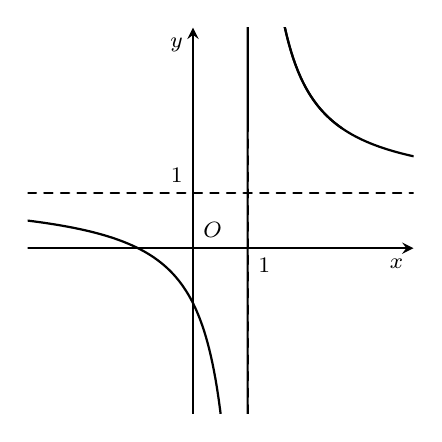
\begin{tikzpicture}[>=stealth, line cap=round, line join=round, font=\footnotesize, thick,scale=0.7]
			\def\xmin{-3}
			\def\xmax{4}
			\def\ymin{-3}
			\def\ymax{4}
			\clip (\xmin,\ymin) rectangle (\xmax,\ymax);
			\draw[->] (\xmin,0)--(0,0)node[above right]{$O$}--(\xmax,0)node[below left]{$x$};
			\draw[->] (0,\ymin)--(0,\ymax)node[below left]{$y$};
			\draw[dashed] (\xmin,1)--(0,1)node[above left]{$1$}--(\xmax,1);
			\draw[dashed] (1,\ymin)--(1,0)node[below right]{$1$}--(1,\ymax);
			\draw[samples=200, domain=1.3:\xmax] plot (\x, {(\x+1)/(\x -1)});
			\draw[samples=200, domain=\xmin:2.7] plot (\x, {(\x+1)/(\x -1)});
		\end{tikzpicture}
	}
\end{ex}%%%%%-----Câu 11-----%%%%%
\begin{ex}%[2H5N1-2]%[Dự án đề TT Toán NH25-26 Đợt 3- Phan Trung Hiếu]%[TT-SGD-Ninh Bình - Ninh BÌnh]%[GVPB: Phạm Văn Long]
	Trong không gian với hệ tọa độ $Oxyz$, cho mặt phẳng $(\alpha)\colon3x+2y-4z+1=0$. Véctơ nào sau đây là một véctơ pháp tuyến của mặt phẳng $(\alpha)$?
	\choice
	{$\vv{n_2}=(2;-4;1)$}
	{$\vv{n_4}=(-4;2;3)$}
	{\True $\vv{n_1}=(3;2;-4)$}
	{$\vv{n_3}=(3;-4;1)$}
	\loigiai{
		Một véctơ pháp tuyến của mặt phẳng $(\alpha)$ là $\vv{n_1}=(3;2;-4)$.
	}
\end{ex}
%%%%%-----Câu 12-----%%%%%
\begin{ex}%[2H5N1-1] %[Dự án đề TT Toán NH25-26 Đợt 3- Phan Trung Hiếu]%[TT-SGD-Ninh Bình - Ninh BÌnh]%[GVPB: Phạm Văn Long]
	Trong không gian với hệ tọa độ $Oxyz$, cho mặt phẳng $(\alpha)\colon x+y+z-4=0$. Điểm nào sau đây thuộc mặt phẳng $(\alpha)$?
	\choice
	{$N(2;3;0)$}
	{$P(4;1;1)$}
	{$Q(2;2;1)$}
	{\True $M(1;2;1)$}
	\loigiai{
		Ta có $1+2+1-4 = 0 $ nên điểm $M(1;2;1)$ thuộc mặt phẳng $(\alpha)$.
	}
\end{ex}

\TNTF
\begin{ex}%[2D4H1-3]%[Dự án đề TT Toán NH 2025-2026 Đợt 3-Lê Minh Thiện Anh]%[Sở GD Ninh Bình - Ninh Bình]%[GVPB: Phạm Văn Long]
	Cho hàm số $f(x) = \cos^2 \dfrac{x}{2}$.
	\choiceTF
	{$\displaystyle \int f(x)\mathrm{\,d}x = \dfrac{x}{2} - \dfrac{1}{2}\sin x + C$}
	{Nếu $F(x)$ là một nguyên hàm của hàm số $f(x)$ trên khoảng $(-\infty; +\infty)$ và thỏa mãn $F(0)=3$ thì $F\left(\dfrac{\pi}{6}\right) = \dfrac{\pi}{12} + \dfrac{11}{4}$}
	{\True $\displaystyle \int\limits_0^{\frac{\pi}{2}} f(x) \mathrm{\,d}x = a + b\pi$ ($a, b \in \mathbb{Q}$), trong đó $a^2 + b = \dfrac{1}{2}$}
	{\True Diện tích của hình phẳng giới hạn bởi đồ thị hàm số $y=f(x)$, $y=x^2-4+\cos^2 \dfrac{x}{2}$ và hai đường thẳng $x=0, x=3$ bằng $\dfrac{23}{3}$}
	\loigiai{
		Ta có $f(x) = \cos^2 \dfrac{x}{2} = \dfrac{1 + \cos x}{2} = \dfrac{1}{2} + \dfrac{1}{2}\cos x$.
		\begin{itemchoice}
			\itemch
			$\displaystyle \int f(x) \mathrm{\,d}x = \int \left(\dfrac{1}{2} + \dfrac{1}{2}\cos x\right) \mathrm{\,d}x = \dfrac{x}{2} + \dfrac{1}{2}\sin x + C$.			
			\itemch 
			Ta có $F(x) = \dfrac{x}{2} + \dfrac{1}{2}\sin x + C$. \\
			Vì $F(0)=3 \Rightarrow \dfrac{0}{2} + \dfrac{1}{2}\sin 0 + C = 3 \Rightarrow C = 3$. \\
			Khi đó $F\left(\dfrac{\pi}{6}\right) = \dfrac{\pi}{12} + \dfrac{1}{2}\sin\dfrac{\pi}{6} + 3 = \dfrac{\pi}{12} + \dfrac{13}{4}$.			
			\itemch 
			$\displaystyle \int\limits_0^{\frac{\pi}{2}} f(x) \mathrm{\,d}x = \left[ \dfrac{x}{2} + \dfrac{1}{2}\sin x \right]\bigg|_0^{\frac{\pi}{2}} = \left(\dfrac{\pi}{4} + \dfrac{1}{2}\right) - 0= \dfrac{1}{2} + \dfrac{1}{4}\pi$. \\
			Suy ra $a = \dfrac{1}{2}$, $b = \dfrac{1}{4}$. Vậy $a^2 + b = \left(\dfrac{1}{2}\right)^2 + \dfrac{1}{4} = \dfrac{1}{2}$.
			\itemch 
			Diện tích $S = \displaystyle \int\limits_0^3 |f(x) - (x^2 - 4 + f(x))|\mathrm{\,d}x = \int\limits_0^3 |4 - x^2|\mathrm{\,d}x$. \\
			$S = \displaystyle \int\limits_0^2 (4-x^2) \mathrm{\,d}x + \int\limits_2^3 (x^2-4) \mathrm{\,d}x = \dfrac{16}{3} + \dfrac{7}{3} = \dfrac{23}{3}$. 
		\end{itemchoice}
	}
\end{ex}

\begin{ex}%[2H2H2-4]%[Dự án đề TT Toán NH 2025-2026 Đợt 3-Lê Minh Thiện Anh]%[Sở GD Ninh Bình - Ninh Bình]%[GVPB: Phạm Văn Long]
	\immini[thm]{Cho hình hộp chữ nhật $ABCD.A'B'C'D'$ có đáy $ABCD$ là hình chữ nhật với $AB=5$, $AD=6$, $AA'=10$ và $G$ là trọng tâm của tam giác $BDA'$. Gắn một hệ tọa độ $Oxyz$ có gốc $O$ trùng với điểm $A$, tia $Ox$ trùng với tia $AB$, tia $Oy$ trùng với tia $AD$, tia $Oz$ trùng với tia $AA'$.
		\choiceTF
		{\True Tọa độ của điểm $C$ là $(5;6;0)$}
		{\True $|\vec{AC} + 2\vec{A'B}| = \sqrt{661}$}
		{Tọa độ điểm $G$ là $\left( 2; \dfrac{5}{3}; \dfrac{10}{3} \right)$}
		{\True $\vec{AG} \cdot \vec{B'C} = -\dfrac{64}{3}$}}
	{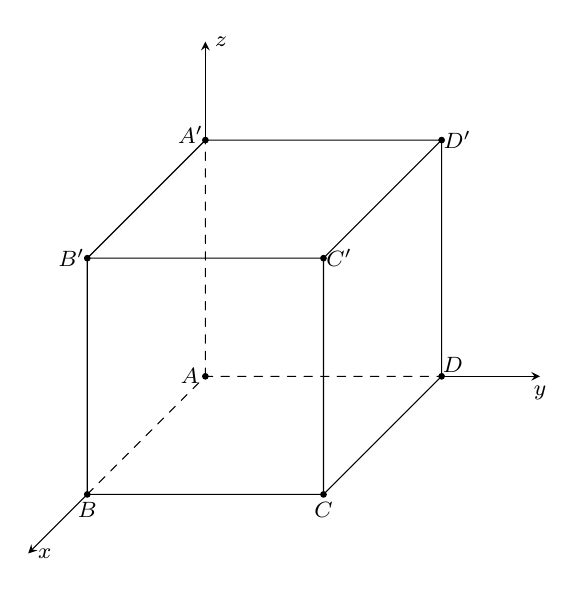
\begin{tikzpicture}[scale=1, font=\footnotesize, line join=round, line cap=round, >=stealth]
			\path
			(0,0) coordinate (B) 
			(3,0) coordinate (C) 
			(1.5,1.5) coordinate (A) 
			(A)+(3,0) coordinate (D);
			\foreach \x in {A,B,C,D}
			\path (\x)+(0,3) coordinate(\x');	
			\draw[dashed] (B)--(A)--(D) (A)--(A');
			\draw(B')--(C')--(D')--(A')--(B')--(B)--(C)--(D)--(D') (C)--(C');
			\draw[->](A')--(1.5,5.75)node[right]{$z$};
			\draw[->](D)--(5.75,1.5)node[below]{$y$};
			\draw[->](B)--(-0.75,-0.75)node[right]{$x$};
			\foreach \p/\g in {B/-90,C/-90,D/45,A/180,B'/180,C'/0,D'/0,A'/160}\draw[fill=black] (\p) circle (1pt)node[shift={(\g:.2)}]{$\p$};
		\end{tikzpicture}
	}
	\loigiai{
		Thiết lập tọa độ các điểm: $A(0;0;0)$, $B(5;0;0)$, $D(0;6;0)$, $C(5;6;0)$, $A'(0;0;10)$, $B'(5;0;10)$.
		\begin{itemchoice}
			\itemch Điểm $C$ có tọa độ $(5;6;0)$.			
			\itemch 
			$\vec{AC} = (5;6;0)$; $\vec{A'B} = (5;0;-10) \Rightarrow 2\vec{A'B} = (10;0;-20)$. \\
			$\vec{u} = \vec{AC} + 2\vec{A'B} = (15; 6; -20)$. \\
			$|\vec{u}| = \sqrt{15^2 + 6^2 + (-20)^2} = \sqrt{225 + 36 + 400} = \sqrt{661}$.
			\itemch 
			$G$ là trọng tâm $\triangle BDA'$\\
			$\Rightarrow x_G = \dfrac{5+0+0}{3} = \dfrac{5}{3}$; $y_G = \dfrac{0+6+0}{3} = 2$; $z_G = \dfrac{0+0+10}{3} = \dfrac{10}{3}$. \\
			Vậy $G\left( \dfrac{5}{3}; 2; \dfrac{10}{3} \right)$.
			\itemch 
			$\vec{AG} = \left( \dfrac{5}{3}; 2; \dfrac{10}{3} \right)$. \\
			$\vec{B'C} = (5-5; 6-0; 0-10) = (0; 6; -10)$. \\
			$\vec{AG} \cdot \vec{B'C} = \dfrac{5}{3} \cdot 0 + 2 \cdot 6 + \dfrac{10}{3} \cdot (-10) = -\dfrac{64}{3}$.
		\end{itemchoice}
	}
\end{ex}


\begin{ex}%[2D1V2-1]%[Dự án đề TT Toán NH25-26-Dot 3-Hồ Hải]%[SGD Ninh Bình - Tỉnh Ninh Bình][GVPB - GV Phạm Văn Long]
	Cho hàm số $f(x) = \mathrm{e}^{x^3-3x^2-9x+2026}$.	
	\choiceTF
	{Hàm số đã cho có đạo hàm là $f^\prime(x) = \mathrm{e}^{x^3-3x^2-9x+2026}$}
	{Hàm số $f(x)$ đồng biến trên khoảng $(-\infty;+\infty)$}
	{Hàm số $f(x)$ có hai cực trị trái dấu}
	{\True Tích giá trị lớn nhất và giá trị nhỏ nhất của hàm số $f(x)$ trên đoạn $\left[-2;2\right]$ bằng $\mathrm{e}^{4035}$}
	\loigiai{
		
		\begin{itemchoice}
			\itemch  Ta có $f^\prime(x) =  (3x^2-6x-9)\mathrm{e}^{x^3-3x^2-9x+2026}$.
			\itemch Xét $f^\prime(x) = 0\Leftrightarrow \hoac{&x= -1\\
				&x= 3.}$\newline
			Bảng biến thiên:
			\begin{center}
				
\begin{tikzpicture}
					\tkzTabInit[nocadre=false,lgt=1.2,espcl=2.5,deltacl=0.6]
					{$x$/0.6,$y'$/0.6,$y$/2}
					{$-\infty$,$-1$,$3$,$+\infty$}
					\tkzTabLine{,+,0,-,0,+,}
					\tkzTabVar
					{-/$0$,+/$\mathrm{e}^{2031}$,-/$\mathrm{e}^{1999}$,+/$+\infty$,}
				\end{tikzpicture}
			\end{center}
			
			\itemch Dựa vào bảng biến thiên, ta có $y_{\max}\cdot y_{\min} = \mathrm{e}^{4030} > 0$.
			\itemch Ta có $-1\in \left[-2;2\right] \Rightarrow \displaystyle\max\limits_{\left[-2;2\right]}f(x) = \mathrm{e}^{2031}$.\newline
			Lại có $f(-2) = \mathrm{e}^{2024}$ và $f(2) = \mathrm{e}^{2004}$.\newline
			Vậy $\displaystyle\max\limits_{\left[-2;2\right]}f(x)\cdot \displaystyle\min\limits_{\left[-2;2\right]}f(x) = \mathrm{e}^{2031}\cdot \mathrm{e}^{2004} = \mathrm{e}^{4035}$.
			
	\end{itemchoice}}
\end{ex}
\begin{ex}%[2H5V1-5]%[Dự án đề TT Toán NH25-26-Dot3-Hồ Hải]%[SGD Ninh Bình - Tỉnh Ninh Bình][GVPB - GV Phạm Văn Long]
	Trong không gian với hệ tọa độ $Oxyz$, cho ba điểm $A(-1;0;2)$, $B(2;2;1)$ và $C(0;-1;4)$.
	\choiceTF
	{Mặt phẳng $(Oxy)$ có phương trình là $x+y=0$}
	{Hình chiếu vuông góc của $B$ lên mặt phẳng $(Oxz)$ là điểm $B'(0;2;1)$}
	{\True Mặt phẳng đi qua $C$ và vuông góc với $AB$ có phương trình là $3x+2y-z+6=0$}
	{\True Gọi $(\alpha)$ là mặt phẳng chứa trục $Ox$ và song song với đường thẳng $AC$. Khoảng cách từ $B$ đến mặt phẳng $(\alpha)$ bằng $\sqrt{5}$}
	\loigiai{
		\begin{itemchoice}
			\itemch Phương trình mặt phẳng $(Oxy)\colon z=0$.
			\itemch Hình chiếu vuông góc của $B$ lên mặt phẳng $(Oxz)$ là $B^\prime (2;0;1)$.
			\itemch $\overrightarrow{AB} = (3;2;-1)$.\newline
			Mặt phẳng đi qua $C(0;-1;4)$ và có $\overrightarrow{AB} = (3;2;-1)$ là một vectơ pháp tuyến có phương trình tổng quát:
			\[3(x-0)+2(y+1)-1(z-4) = 0 \Leftrightarrow 3x+2y-z+6=0\]
			\itemch Vì mặt phẳng $(\alpha)$ chứa trục $Ox$ và song song với đường thẳng $AC$ nên có hai vectơ chỉ phương là $\overrightarrow{i} = (1;0;0)$ và $\overrightarrow{AC} =(1;-1;2)$.\newline
			Vectơ pháp tuyến: $\overrightarrow{n} = [\overrightarrow{i}, \overrightarrow{AC}] = (0;-2;-1)$.\newline
			Mặt phẳng $(\alpha)$ qua $O(0;0;0)$ và nhận $\overrightarrow{n} = (0;-2;-1)$ là một vectơ pháp tuyến có phương trình tổng quát:
			\[ -2y-z=0\Leftrightarrow 2y+z=0\]
			Khoảng cách từ điểm $B$ đến mặt phẳng $(\alpha)$ 
			$$\mathrm{d}(B,(\alpha)) = \dfrac{\left|0\cdot2 +2\cdot 2 +1\cdot 1 \right|}{\sqrt{0^2+2^2+1^2}} = \dfrac{5}{\sqrt{5}}=\sqrt{5}.$$
	\end{itemchoice}}
\end{ex}

\TNSA
\begin{ex}%[2H5V2-8]%[Dự án đề TT Toán NH25-26 đợt 3-Nguyễn Hoài Nam]%[SGD Ninh Bình-Ninh Bình]%[GVPB: Phạm Văn Long]
	Trong không gian với hệ tọa độ $Oxyz$ (đơn vị trên mỗi trục là km), một Radar phát hiện một chiếc máy bay di chuyển trên một đường thẳng với tốc độ và hướng bay không đổi. Máy bay bay từ điểm $A(712;200;6)$ đến điểm $B(802;220;8)$ trong $8$ phút và trong $4$ phút tiếp theo máy bay có vị trí là điểm $C(x;y;z)$. Giá trị $x+y+z$ bằng bao nhiêu?
	\shortans{$1\,086$}
	\loigiai{
		Ta có véc-tơ $\overrightarrow{AB}=(90;20;2)$. Đây là quãng đường máy bay đi được trong $8$ phút.\\
		Vì máy bay di chuyển trên một đường thẳng với tốc độ và hướng không đổi, nên trong $4$ phút tiếp theo, máy bay di chuyển một quãng đường tương ứng với véc-tơ $\overrightarrow{BC}$.\\
		Do thời gian $4$ phút bằng $\dfrac{1}{2}$ thời gian $8$ phút, ta có mối liên hệ giữa các véc-tơ dịch chuyển
		$$\overrightarrow{BC} = \dfrac{1}{2} \overrightarrow{AB} = \left(\dfrac{90}{2};\dfrac{20}{2};\dfrac{2}{2} \right) = (45;10;1).$$
		Tọa độ điểm $C$ được xác định bởi
		$\heva{&x=x_B+45=802+45=847\\ &y=y_B+10=220+10=230\ &z =z_B+1=8+1=9}  \Rightarrow C(847;230;9)$.\\
		Giá trị biểu thức cần tìm là $x+y+z=847+230+9=1 \,086$.
	}
\end{ex}

\begin{ex}%[2D4C3-2]%[Dự án đề TT Toán NH25-26 đợt 3-Nguyễn Hoài Nam]%[SGD Ninh Bình-Ninh Bình]%[GVPB: Phạm Văn Long]
	Trong hình bên là một chiếc đồng hồ treo tường cao cấp được thiết kế có phần ở giữa (phần tô đậm) dát vàng. Phần này được thiết kế như sau: 
	\begin{itemize}
		\item Vẽ hình lục giác đều $ABCDEF$ tâm $O$ và có cạnh bằng $4$ cm;
		\item Vẽ parabol $(C_1)$ tiếp xúc với các đường thẳng $OA$, $OB$ lần lượt tại $A$ và $B$;
		\item Tương tự vẽ parabol $(C_2)$ tiếp xúc với các đường thẳng $OB$, $OC$ lần lượt tại $B$ và $C$; parabol $(C_3)$ tiếp xúc với các đường thẳng $OC$, $OD$ lần lượt tại $C$ và $D$; \ldots; parabol $(C_6)$ tiếp xúc với các đường thẳng $OF$, $OA$ lần lượt tại $F$ và $A$.
	\end{itemize}
	Hình phẳng $(H)$ được giới hạn bởi sáu parabol $(C_1)$, $(C_2)$, $(C_3)$, $(C_4)$, $(C_5)$, $(C_6)$ (phần tô đậm) là phần sẽ được dát vàng. Hỏi phần dát vàng này có diện tích bằng bao nhiêu centimét vuông (không làm tròn kết quả các phép tính trung gian, chỉ làm tròn kết quả cuối cùng đến hàng phần chục)?
	\begin{center}
		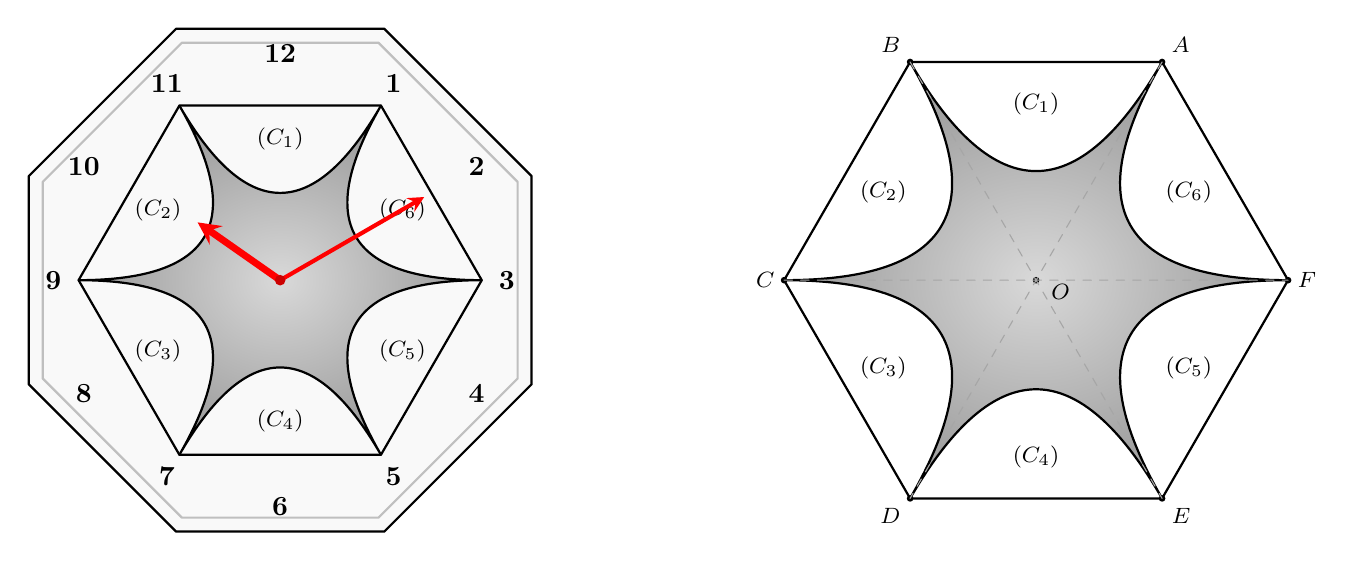
\begin{tikzpicture}[>=stealth, line join=round, line cap=round, font=\footnotesize, scale=0.8]
			
			% ==========================================
			% HÌNH 1: CHIẾC ĐỒNG HỒ THỰC TẾ (BÊN TRÁI)
			% ==========================================
			\begin{scope}[shift={(0,0)},scale=0.8]
				\coordinate (O) at (0,0);
				
				% 1. Vẽ viền bát giác đều bao bên ngoài (2 lớp)
				\draw[thick, fill=gray!5] 
				(22.5:5.4) -- (67.5:5.4) -- (112.5:5.4) -- (157.5:5.4) -- 
				(202.5:5.4) -- (247.5:5.4) -- (292.5:5.4) -- (337.5:5.4) -- cycle;
				\draw[thick, gray!50] 
				(22.5:5.1) -- (67.5:5.1) -- (112.5:5.1) -- (157.5:5.1) -- 
				(202.5:5.1) -- (247.5:5.1) -- (292.5:5.1) -- (337.5:5.1) -- cycle;
				
				% Tính toán tọa độ các đỉnh lục giác đều bên trong (R=4)
				\foreach \i/\a in {1/60, 2/120, 3/180, 4/240, 5/300, 6/360} {
					\coordinate (V\i) at (\a:4);
				}
				
				% Vẽ các đường chéo và cạnh lục giác
				\draw[thin, gray!70] (V1)--(V4) (V2)--(V5) (V3)--(V6);
				\draw[thick] (V1)--(V2)--(V3)--(V4)--(V5)--(V6)--cycle;
				
				% Tô màu và vẽ 6 parabol phần lõi
				\shade[inner color=gray!30, outer color=gray!80, draw=black, thick] 
				(V1) .. controls (60:1.333) and (120:1.333) .. (V2)
				.. controls (120:1.333) and (180:1.333) .. (V3)
				.. controls (180:1.333) and (240:1.333) .. (V4)
				.. controls (240:1.333) and (300:1.333) .. (V5)
				.. controls (300:1.333) and (360:1.333) .. (V6)
				.. controls (360:1.333) and (60:1.333) .. (V1);
				
				% Ký hiệu (C1), (C2)...
				\node at (90:2.8) {$(C_1)$};
				\node at (150:2.8) {$(C_2)$};
				\node at (210:2.8) {$(C_3)$};
				\node at (270:2.8) {$(C_4)$};
				\node at (330:2.8) {$(C_5)$};
				\node at (30:2.8) {$(C_6)$};
				
				% 2. Các cột số của đồng hồ (1 -> 12)
				\foreach \num/\angle in {1/60, 2/30, 3/0, 4/330, 5/300, 6/270, 7/240, 8/210, 9/180, 10/150, 11/120, 12/90} {
					\node[font=\bfseries\normalsize] at (\angle:4.5) {\num};
				}
				
				% 3. Kim đồng hồ (10 giờ 10 phút)
				% Kim phút chỉ ngay số 2 (góc 30 độ)
				\draw[->, red, line width=1.5pt] (0,0) -- (30:3.3); 
				% Kim giờ nhích qua số 10 một chút (10 giờ 10 phút -> góc 145 độ)
				\draw[->, red, line width=2.5pt] (0,0) -- (145:2.0);
				% Trục kim đồng hồ
				\fill[red!80!black] (0,0) circle (3pt);
			\end{scope}
			
			% ==========================================
			% HÌNH 2: MÔ HÌNH TOÁN HỌC GỐC (BÊN PHẢI)
			% ==========================================
			\begin{scope}[shift={(12,0)}] % Tịnh tiến sang phải 12 đơn vị để cách hình 1 tầm ~2cm
				\coordinate (O) at (0,0);
				
				% Tính toán tọa độ các đỉnh lục giác đều bán kính R=4
				\foreach \i/\a in {1/60, 2/120, 3/180, 4/240, 5/300, 6/360} {
					\coordinate (V\i) at (\a:4);
				}
				
				% Vẽ các đường chéo (sử dụng nét đứt - dashed) và cạnh lục giác
				
				\draw[thick] (V1)--(V2)--(V3)--(V4)--(V5)--(V6)--cycle;
				
				% Tô màu và vẽ 6 parabol bằng lệnh controls.
				\shade[inner color=gray!30, outer color=gray!80, draw=black, thick] 
				(V1) .. controls (60:1.333) and (120:1.333) .. (V2)
				.. controls (120:1.333) and (180:1.333) .. (V3)
				.. controls (180:1.333) and (240:1.333) .. (V4)
				.. controls (240:1.333) and (300:1.333) .. (V5)
				.. controls (300:1.333) and (360:1.333) .. (V6)
				.. controls (360:1.333) and (60:1.333) .. (V1);
				
				% Ký hiệu (C1), (C2)...
				\node at (90:2.8) {$(C_1)$};
				\node at (150:2.8) {$(C_2)$};
				\node at (210:2.8) {$(C_3)$};
				\node at (270:2.8) {$(C_4)$};
				\node at (330:2.8) {$(C_5)$};
				\node at (30:2.8) {$(C_6)$};
				
				% Tên các đỉnh
				\foreach \i/\n/\pos in {1/A/above right, 2/B/above left, 3/C/left, 4/D/below left, 5/E/below right, 6/F/right} {
					\fill (V\i) circle (1.5pt) node[\pos] {$\n$};
				}
				\fill (O) circle (1.5pt) node[below right, xshift=2pt, yshift=2pt] {$O$};
				\draw[dashed, thin, gray!70] (V1)--(V4) (V2)--(V5) (V3)--(V6);
			\end{scope}
		\end{tikzpicture}
	\end{center}
	\shortans{$13{,}9$}
	\loigiai{\immini[thm]{Chọn hệ trục tọa độ $Oxy$ sao cho gốc $O(0;0)$, tia $Ox$ trùng với tia $OF$, tia $Oy$ là tia phân giác của góc $\widehat{AOB}$ (tham khảo hình vẽ bên).\\
			Do $ABCDEF$ là lục giác đều cạnh bằng $4$ cm nên $OA=OB=OC=OD=OE=OF=4$ cm. Suy ra, $A=(4\cos 60^\circ;4\sin 60^\circ)=(2;2\sqrt{3})$ và\break $B=(4\cos 120^\circ;4\sin 120^\circ)=(-2;2\sqrt{3})$.\\
			Do prabol $(C_1)$ tiếp xúc với $OA$ và $OB$ nên parabol $(C_1)$ nhận $Oy$ làm trục đối xứng, do đó phương trình parabol $(C_1)$ có dạng $y=a x^2+b$. Suy ra, $y'=2a x$. \\
			Đường thẳng $OA$ có hệ số góc $k_A=\tan 60^\circ=\sqrt{3}$. Do $(C_1)$ tiếp xúc với $OA$ tại $A(2;2\sqrt{3})$ nên 
			$$y'(2)=k_A\Leftrightarrow 4a=\sqrt{3}\Leftrightarrow a=\dfrac{\sqrt{3}}{4}.$$
		}{\begin{tikzpicture}[scale=0.8, font=\footnotesize, line join=round, line cap=round, >=stealth]
				\coordinate (O) at (0,0);
				
				% Tính toán tọa độ các đỉnh lục giác đều bán kính R=4
				\foreach \i/\a in {1/60, 2/120, 3/180, 4/240, 5/300, 6/360} {
					\coordinate (V\i) at (\a:4);
				}
				
				% Vẽ các đường chéo (sử dụng nét đứt - dashed) và cạnh lục giác
				
				\draw[thick] (V1)--(V2)--(V3)--(V4)--(V5)--(V6)--cycle;
				
				% Tô màu và vẽ 6 parabol bằng lệnh controls.
				\shade[inner color=gray!30, outer color=gray!80, draw=black, thick] 
				(V1) .. controls (60:1.333) and (120:1.333) .. (V2)
				.. controls (120:1.333) and (180:1.333) .. (V3)
				.. controls (180:1.333) and (240:1.333) .. (V4)
				.. controls (240:1.333) and (300:1.333) .. (V5)
				.. controls (300:1.333) and (360:1.333) .. (V6)
				.. controls (360:1.333) and (60:1.333) .. (V1);
				
				% Ký hiệu (C1), (C2)...
				\node at (80:2.8) {$(C_1)$};
				\node at (150:2.8) {$(C_2)$};
				\node at (210:2.8) {$(C_3)$};
				\node at (260:2.8) {$(C_4)$};
				\node at (330:2.8) {$(C_5)$};
				\node at (30:2.8) {$(C_6)$};
				
				% Tên các đỉnh
				\foreach \i/\n/\pos in {1/A/above right, 2/B/above left, 3/C/above left, 4/D/below left, 5/E/below right, 6/F/above right} {
					\fill (V\i) circle (1.5pt) node[\pos] {$\n$};
				}
				\fill (O) circle (1.5pt) node[below right, xshift=2pt, yshift=2pt] {$O$};
				\draw[dashed, thin, gray!70] (V1)--(V4) (V2)--(V5) (V3)--(V6);
				\draw[-stealth] ($(O)!1.2!(V3)$)--($(O)!1.3!(V6)$) node [above] {$x$};
				\draw[-stealth] ($(O)!1.1!-90:(V6)$)--($(O)!1.2!90:(V6)$) node [right] {$y$};
		\end{tikzpicture}}
		Mặt khác, $A(2;2\sqrt{3})\in (C_1)$ nên $4a+b=2\sqrt{3}$, suy ra $b=2\sqrt{3}-4a=2\sqrt{3}-\sqrt{3}=\sqrt{3}$.\\
		Do đó, $(C_1)\colon y=\dfrac{\sqrt{3}}{4}x^2+\sqrt{3}$.\\
		Diện tích phần giới hạn bởi đường thẳng $AB$ và parabol $(C_1)$ là
		$$\mathrm{S}_1=\int\limits_{-2}^2 \left(2\sqrt{3}-\dfrac{\sqrt{3}}{4}x^2-\sqrt{3}\right)\mathrm{\,d}x=\int\limits_{-2}^2 \left(\sqrt{3}-\dfrac{\sqrt{3}}{4}x^2\right)\mathrm{\,d}x=\left.\left(\sqrt{3}x-\dfrac{\sqrt{3}}{12}x^3\right)\right|_{-2}^2=\dfrac{8\sqrt{3}}{3}.$$
		Suy ra, diện tích phần hình phẳng giới hạn bởi parabol $(C_1)$, $OA$ và $OB$ là 
		$$\mathrm{S}=\mathrm{S}_{OAB}-\mathrm{S}_1=\dfrac{4^2\sqrt{3}}{4}-\dfrac{8\sqrt{3}}{3}=\dfrac{4\sqrt{3}}{3}.$$
		Diện tích hình phẳng $(H)$ là
		$$\mathrm{S}_H=6\mathrm{S}=6\cdot\dfrac{4\sqrt{3}}{3}=8\sqrt{3}\approx 13{,}9.$$}
\end{ex}
%%=======Câu 3=======%%
\begin{ex}%[2H5V1-5]%[Dự án đề TT Toán NH25-26-Dot-3-Trung Kien]%[SGD Ninh Bình Lần 2 - Ninh Bình]%[GVPB-Phạm Văn Long]
	Trong không gian $Oxyz$ (đơn vị trên mỗi trục tọa độ là mét), một ngôi nhà (xem hình vẽ bên) có sàn nhà nằm ngang trên mặt phẳng $(\alpha) \colon y - z - 5 = 0$. Hai mái nhà (coi như là hai phần mặt phẳng) lần lượt nằm trên các mặt phẳng $(P) \colon 2x - 3y + z - 6 = 0$, $(Q) \colon 2x + y - 3z + 10 = 0$. Hỏi chiều cao của ngôi nhà tính từ nóc nhà (điểm cao nhất của mái nhà) đến sàn nhà là bao nhiêu mét (không làm tròn kết quả các phép tính trung gian, chỉ làm tròn kết quả cuối cùng đến hàng phần trăm)?
	\begin{center}
		\begin{tikzpicture}[scale=1, font=\footnotesize, line join=round, line cap=round, >=stealth, transform shape]
			\path 
			(-1.8,1.2) coordinate (C)
			(2.6,1.2) coordinate (E)
			(0.37,2.45) coordinate (D)
			(-1.2,2.4) coordinate (G)
			(0.37,3.26) coordinate (F)
			(2,2.4) coordinate (H)
			($(C)!0.15!(D)$) coordinate (A)
			($(E)!0.15!(D)$) coordinate (B)
			($(A)+(0,-2)$) coordinate (M)
			($(B)+(0,-2)$) coordinate (N)
			($(C)!0.65!(D)$) coordinate (A1)
			($(E)!0.65!(D)$) coordinate (B1)
			($(A1)!0.5!(B1)$) coordinate (O)
			($(M)!0.3!(N)$) coordinate (M1)
			($(M)!0.7!(N)$) coordinate (N1)
			;
			\draw (C)--(D)--(E) (G)--(F)--(H) (C)--(G) (E)--(H) (D)--(F)
			(A)--(B) (A)--(M) (B)--(N)--(M)
			;
			\draw(A1)--($(A1)+(0,-0.62)$) coordinate (A2) (B1)--($(B1)+(0,-0.62)$)coordinate (B2);
			\draw[pattern=dots] ($(O)+(0,-0.2)$) circle (8pt);
			\draw[pattern=horizontal lines] (A1)--(A)--(A2)--cycle;
			\draw[pattern=horizontal lines] (B1)--(B)--(B2)--cycle;
			\draw[pattern=horizontal lines] (M1)--($(M1)+(0,1.5)$)--($(N1)+(0,1.5)$)--(N1);
			
			\fill[gray!30] (A)--(B)--($(B)+(0,-0.1)$)--($(A)+(0,-0.1)$);
			\draw ($(A)+(0,-0.1)$)--($(B)+(0,-0.1)$);
			\draw (-1.8,0)coordinate(a)--(-3.5,-1.5)coordinate(b)--(1.5,-1.5)coordinate(c);
			\pic[draw,thin,angle radius=9mm,"$\alpha$"] {angle=c--b--a};
		\end{tikzpicture}
	\end{center}
	\shortans[oly]{$6{,}36$}
	\loigiai{
		Gọi $d$ là giao tuyến của hai mặt phẳng $(P)$ và $(Q)$. Khi đó $d \parallel (\alpha)$.\\
		Chọn điểm $M$ tùy ý thuộc $d$, tọa độ điểm $M$ là nghiệm của hệ phương trình
		$$\heva{&2x - 3y + z - 6 = 0\\&2x + y - 3z + 10 = 0.}$$
		Chọn $x=0$, ta được hệ $\heva{&- 3y + z - 6 = 0\\&y - 3z + 10 = 0} \Leftrightarrow \heva{&y=-1\\&z=3.}$\\
		Nên $M(0;-1;3)$.\\
		Chiều cao ngôi nhà tính từ nóc nhà bằng khoảng cách từ điểm $M$ đến mặt phẳng $(\alpha)$,
		$$\mathrm{d}(M,(\alpha))=\dfrac{|y_M-z_M-5|}{\sqrt{1^2+(-1)^2}}=\dfrac{9\sqrt{2}}{2} \approx 6{,}36.$$
		
	}
\end{ex}

%=======Câu 4=======%%
\begin{ex}%[2D1C3-6]%[Dự án đề TT Toán NH25-26-Dot-3-Trung Kien]%[SGD Ninh Bình Lần 2 - Ninh Bình]%[GVPB-Phạm Văn Long]
	Ông chủ của một ngôi nhà muốn làm một chiếc thang cứu hộ (coi như một đoạn thẳng) để sử dụng khi có nguy hiểm xảy ra. Khi chiếc thang được sử dụng thì một đầu của nó sẽ tiếp đất và một đầu còn lại sẽ đặt vào bức tường của ngôi nhà. Chiếc thang này được thiết kế để nó đứng dưới đất vươn qua hàng rào tựa vào ngôi nhà (tham khảo hình vẽ bên). Hàng rào cao $2{,}88$ mét được đặt song song và cách bức tường của ngôi nhà một khoảng bằng $1{,}8$ mét. Hỏi chiều dài ngắn nhất của chiếc thang bằng bao nhiêu mét (không làm tròn kết quả các phép tính trung gian, chỉ làm tròn kết quả cuối cùng đến hàng phần trăm)?
	\begin{center}
		\begin{tikzpicture}[scale=0.7, font=\footnotesize, line join=round, line cap=round, >=stealth, transform shape]
			\draw[fill=blue!30!white] (0,0)--(5,1)--(5,4)--(0,3)--cycle;
			\draw[fill=blue!30!black]
			(0,0)--(-3,1)--(-3,4)--(0,3)--cycle;			
			\draw (1.25,0.25)--++(0,3)
			(2.5,0.5)--++(0,3)
			(3.75,0.75)--++(0,3); 
			\draw[fill=yellow] (-0.53,2.89)--(5.53,4.11)--(2.01,5.63)--cycle;			
			\tikzset{hangrao/.pic={
					\draw[fill=gray] (0,0)--++(5/20,1/20)--++(0,2)--++(-5/40,1/20)--++(-5/40,-1/20)--cycle;
			}}
			\draw[fill=gray] (1,0)--(6,1)--++(0,-0.2)--++(-5,-1)--cycle;
			\foreach \x in {0,2,4,...,20}{\pic at (1+\x/4,-1+\x/20){hangrao};}		
			\draw[fill=yellow!70!black] (2.01,5.63)--(-0.53,2.89)--(-3.53,3.89)--(-0.66,6.52)--cycle;			
			\draw[line width=2pt] (2.5,2.99)--(4.26,-1)
			(2.98,3.09)--(4.74,-0.89)
			\foreach \x in {0.1,0.2,0.3,0.4,0.5,0.6,0.7,0.8,0.9}{
				($(2.5,2.99)!\x!(4.26,-1)$)--++(0.48,0.1)};
		\end{tikzpicture}
	\end{center}
	\shortans[oly]{}
	\loigiai{
		\begin{center}
			\begin{tikzpicture}[scale=1, font=\footnotesize, line join=round, line cap=round, >=stealth]
				\draw (0,0)--(4,0)--(0,3.84)--cycle
				(1.5,0)--(1.5,2.4);
				\fill 
				(0,0)node[below left]{$A$} circle (1pt)
				(4,0)node[below right]{$B$} circle (1pt)
				(0,3.84)node[above]{$C$} circle (1pt)
				(1.5,0)node[below]{$K$} circle (1pt)
				(1.5,2.4)node[above]{$H$} circle (1pt);
			\end{tikzpicture}
		\end{center}
		Minh hoạ bài toán như trên, với $B$ là vị trí đặt thang trên mặt đất, khoảng cách từ nhà đến hàng rào là $AK=1{,}8$ m và hàng rào có độ cao $HK=2{,}88$ m.\\
		Đặt $KB=x$, $x>0$ (m). Vì $HK \parallel AC$ nên $\dfrac{HK}{AC}=\dfrac{KB}{AB}$. Suy ra
		$$AC = AB \cdot \dfrac{HK}{KB} = (x+1{,}8) \cdot \dfrac{2{,}88}{x}.$$
		Xét tam giác $ABC$ vuông tại $A$, ta có
		$$BC^2= AC^2 + AB^2=\dfrac{2{,}88^2}{x^2}\cdot(x+1{,}8)^2 + (x+1{,}8)^2.$$
		Đặt $a=1{,}8$ và $b=2{,}88$, ta được
		\begin{eqnarray*}
			BC^2	&=& \dfrac{b^2}{x^2}\cdot(x+a)^2 + (x+a)^2\\
			&=& x^2 + \dfrac{2ab^2}{x} + 2ax + \dfrac{a^2b^2}{x^2} + a^2 + b^2\\
			&=& \left(x^2 + \dfrac{ab^2}{x} + \dfrac{ab^2}{x}\right) + \left(ax + ax + \dfrac{a^2b^2}{x^2}\right)+a^2+b^2\\
			&\ge& 3\sqrt[3]{a^2b^4}	+ 3\sqrt[3]{a^4b^2}	+a^2+b^2\\
			&\approx& 43{,}02.
		\end{eqnarray*}
		Dấu ``='' xảy ra khi $x^3=ab^2$.\\
		Vậy $BC$ nhỏ nhất bằng $\sqrt{43{,}02}\approx6{,}56$.}
\end{ex}
\begin{ex}%[2D3K3-3]%[Dự án đề TT Toán NH25-26 Đợt 3-Đỗ Chí Tâm]%[SGD Ninh Bình-Ninh Bình]%[GVPB:Phạm Văn Long]
	Có một hình phẳng $(H)$ (phần tô đậm trong hình vẽ bên) được tạo ra bằng cách vẽ một hình vuông có cạnh bằng $4$. Sau đó, ở bốn góc hình vuông đó vẽ bốn đường cong đều có tính chất là: tích khoảng cách từ một điểm bất kì thuộc mỗi đường cong đó đến hai trục đối xứng $d_1, d_2$ của hình vuông bằng $2$. Khi cho hình phẳng $(H)$ quay quanh trục $d_1$ ta sẽ thu được một vật thể tròn xoay, thể tích vật thể tròn xoay đó bằng bao nhiêu (không làm tròn kết quả các phép tính trung gian, chỉ làm tròn kết quả cuối cùng đến hàng phần chục)? 
	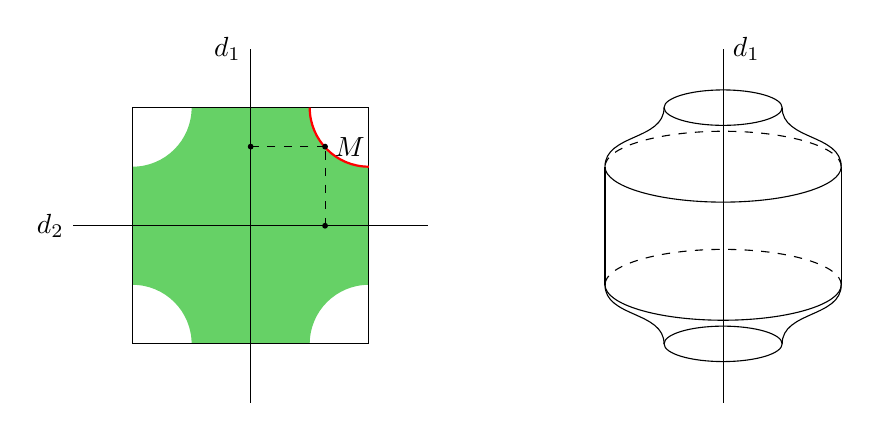
\begin{tikzpicture}[>=stealth, scale=1.5]
		
		% --- HÌNH 1: HÌNH PHẲNG ---
		\begin{scope}[xshift=0cm]
			% Tô màu xanh cho hình phẳng
			\fill[green!70!black!60] (0.5,1) -- (-0.5,1) 
			arc (0:-90:0.5) -- (-1,0.5) -- (-1,-0.5) 
			arc (90:0:0.5) -- (-0.5,-1) -- (0.5,-1) 
			arc (180:90:0.5) -- (1,-0.5) -- (1,0.5) 
			arc (270:180:0.5) -- cycle;
			
			% Vẽ khung hình vuông bao quanh
			\draw (-1,-1) rectangle (1,1);
			
			% Vẽ các trục đối xứng
			\draw (-1.5,0) -- (1.5,0) node[left] at (-1.5,0) {$d_2$};
			\draw (0,-1.5) -- (0,1.5) node[left] at (0,1.5) {$d_1$};
			
			% Chú thích "trục đối xứng"
			%			\node[right, scale=0.8] at (0,1.3) {truc doi xung};
			%			\node[right, scale=0.8] at (1,0.5) {truc doi xung};
			
			% Vẽ cung tròn màu đỏ và điểm M
			\draw[red, thick] (1,0.5) arc (270:180:0.5);
			%\fill (0.65, 0.86) circle (0.7pt) node[above right] {$M$};
			
			% Vẽ đường dóng từ M
			\draw[dashed] (0.63, 0.67) -- (0, 0.67);
			\draw[dashed] (0.63, 0.63) -- (0.63, 0);
			\fill (0, 0.67) circle (0.7pt);
			\fill (0.63, 0) circle (0.7pt);
			\fill (0.63, 0.67) circle (0.7pt) node[right]{$M$};
		\end{scope}
		
		% --- HÌNH 2: VẬT THỂ XOAY ---
		\begin{scope}[xshift=4cm]
			% Trục d1
			\draw (0,-1.5) -- (0,1.5) node[right] {$d_1$};
			
			% Các đường elip (mặt cắt ngang)
			\draw (0,1) ellipse (0.5 and 0.15); % Đỉnh trên
			\draw[dashed] (1,0.5) arc (0:180:1 and 0.3); % Giữa trên (phần khuất)
			\draw (1,0.5) arc (0:-180:1 and 0.3);        % Giữa trên (phần thấy)
			
			\draw[dashed] (1,-0.5) arc (0:180:1 and 0.3); % Giữa dưới (phần khuất)
			\draw (1,-0.5) arc (0:-180:1 and 0.3);        % Giữa dưới (phần thấy)
			
			\draw (0,-1) ellipse (0.5 and 0.15); % Đáy dưới
			
			% Vẽ các đường sinh bên ngoài
			\draw (-1, 0.5) -- (-1, -0.5); % Đường thẳng thân trụ trái
			\draw (1, 0.5) -- (1, -0.5);   % Đường thẳng thân trụ phải
			
			% Cung tròn tạo hình thắt (phần trên và dưới)
			\draw (-0.5, 1) to[out=270, in=90] (-1, 0.5);
			\draw (0.5, 1) to[out=270, in=90] (1, 0.5);
			\draw (-1, -0.5) to[out=270, in=90] (-0.5, -1);
			\draw (1, -0.5) to[out=270, in=90] (0.5, -1);
			
			% Đường trục đứt nét bên trong
			\draw[dashed] (0, 1) -- (0, -1);
		\end{scope}
		
	\end{tikzpicture}
	
	\shortans[oly]{$37{,}7$}
	\loigiai{
		\immini[thm]{
			Xét một phần đường cong ở cung phân từ thứ nhất trong hệ trục tọa độ $Oxy$ như hình.\\
			Vì $d(M, Ox)\cdot d(M,Oy)=2\Leftrightarrow y_M\cdot x_M=2$,\\
			nên $M\in (C): y=\dfrac{2}{x}$.\\
			$(C)$ giao với đường thẳng $y=2$ tai điểm $N(1; 2)$.\\
			Thể tích do $\dfrac{1}{4}$ hình $(H)$ (phần thuộc góc phần tư thứ nhất) quay quanh trục $Ox$ là\\
			$V_1=\displaystyle\pi\int_{0}^{1}2^2dx+\pi\int_{1}^{2}\dfrac{4}{x^2}dx=6\pi.$\\
			Vậy thể tích khối tròn xoay khi cho hình $(H)$ quay quanh trục $d_1$ là\\
			\hspace*{2cm}$V=2V_1=12\pi\approx 37{,}7$.
		}{
			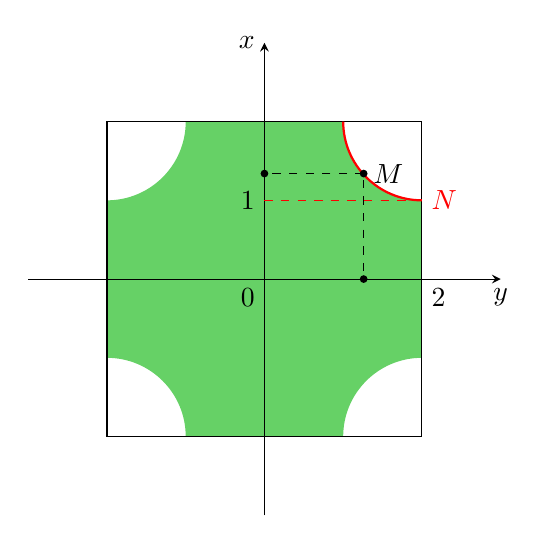
\begin{tikzpicture}[>=stealth, scale=2]
				
				% --- HÌNH 1: HÌNH PHẲNG ---
				\begin{scope}[xshift=0cm]
					% Tô màu xanh cho hình phẳng
					\fill[green!70!black!60] (0.5,1) -- (-0.5,1) 
					arc (0:-90:0.5) -- (-1,0.5) -- (-1,-0.5) 
					arc (90:0:0.5) -- (-0.5,-1) -- (0.5,-1) 
					arc (180:90:0.5) -- (1,-0.5) -- (1,0.5) 
					arc (270:180:0.5) -- cycle;
					
					% Vẽ khung hình vuông bao quanh
					\draw (-1,-1) rectangle (1,1);
					
					% Vẽ các trục đối xứng
					\draw[->] (-1.5,0) -- (1.5,0) node[below]{$y$};
					\draw[->] (0,-1.5) -- (0,1.5) node[left]{$x$};
					\draw[dashed, red](0,0.5)--(1,0.5) node[right]{$N$};
					
					% Chú thích "trục đối xứng"
					%			\node[right, scale=0.8] at (0,1.3) {truc doi xung};
					%			\node[right, scale=0.8] at (1,0.5) {truc doi xung};
					
					% Vẽ cung tròn màu đỏ và điểm M
					\draw[red, thick] (1,0.5) arc (270:180:0.5);
					%\fill (0.65, 0.86) circle (0.7pt) node[above right] {$M$};
					
					% Vẽ đường dóng từ M
					\draw[dashed] (0.63, 0.67) -- (0, 0.67);
					\draw[dashed] (0.63, 0.63) -- (0.63, 0);
					\fill (0, 0.67) circle (0.7pt);
					\fill (0.63, 0) circle (0.7pt);
					\fill (0.63, 0.67) circle (0.7pt) node[right]{$M$};
					\node[below right] at (1,0){$2$};
					\node[below left] at (0,0){$0$};
					\node[left] at(0,0.5){$1$};
				\end{scope}		
			\end{tikzpicture}
		}
	}
\end{ex}

\begin{ex}%[0D2V2-3]%[Dự án đề TT Toán NH25-26 Đợt 3-Đỗ Chí Tâm]%[SGD Ninh Bình-Ninh Bình]%[GVPB:Phạm Văn Long]
	Một công ty $A$ chuyên sản xuất giấy đã nhận được một đơn đặt hàng theo tháng từ đối tác $B$, mỗi tháng công ty $A$ phải cung cấp cho đối tác $B$ ít nhất $2800$ kg giấy in và $2400$kg giấy carton. Công ty $A$ sử dụng hai loại nguyên liệu là gỗ keo và gỗ bạch đàn. Từ một tấn gỗ keo sản xuất ra được $200$ kg giấy in và $300$ kg giấy carton; từ một tấn gỗ bạch đàn sản xuất ra được $300$ kg giấy in và $150$ kg giấy carton. Một tấn gỗ keo có giá là $1{,}2$ triệu đồng và một tấn gỗ bạch đàn có giá là $1{,}5$ triệu đồng. Biết mỗi tháng cơ sở cung cấp nguyên liệu chỉ cung cấp không quá $9$ tấn gỗ keo và không quá $10$ tấn gỗ bạch đàn. Số tiền nhỏ nhất mà công ty $A$ cần dùng mỗi tháng để mua nguyên liệu là bao nhiêu triệu đồng? 
	\shortans[oly]{$15$}
	\loigiai{
		\immini[thm]{
			Gọi $x$, $y$ lần lượt là số tấn gỗ keo và gỗ bạch đàn mà công ty $A$ cần dùng để sản xuất giấy cho đối tác $B$.\\
			Theo đề, ta có $\heva{&0\le x\le 9, 0\le y\le 10\\&200x+300y\ge 2800\\&300x+150y\ge 2400}\\$
			$\Leftrightarrow \heva{&0\le x\le 9, 0\le y\le 10\\&x+1{,}5y\ge 14\\&2x+y\ge 16}$\\
			$d_1: x+1{,}5y-14=0,\,\, d_2:2x+y-16=0$.\\
			$A(3;10), B(9;10), C\left(9;\dfrac{10}{3} \right), D(5;6).$\\
			Số tiền công ty $A$ dùng để mua nguyên vật liệu là\\
			$F(x;y)=1{,}2x+1{,}5y$ (triệu đồng).\\
			$F(A)=18{,}6, F(B)=25{,}8,$\\
			$ F(C)=15{,}8, F(D)=15$.\\
			Vậy số tiền thấp nhất mà công ty $A$ cần dùng để mua nguyên liệu mỗi tháng là $15$ (triệu đồng).
		}{
			\begin{tikzpicture}[scale=0.8, font=\footnotesize, line join=round, line cap=round, >=stealth]
				\draw[->] (-2,0)--(0,0)node[below left]{$O$}--(7.5,0)node[right]{$x$};
				\draw[->] (0,-2)--(0,8.2)node[right]{$y$};
				\clip (-2,-2) rectangle (7.6,8.2);
				\draw[red, thick] (-1,5.333)node[above]{$d_1$}--(7.5,-0.333);
				\draw[blue, thick] (0,8)--(5,-2); \node[right] at (4.7,-1.8) {$d_2$};
				\draw (-1,5)--(7,5) node[above]{$y=10$};
				\draw (4.5,-1)--(4.5,8) node[right]{$x=9$};
				\fill[pattern = north east lines, pattern color = black,opacity=0.45] (-1,5)--(7,5)--(7,9)--(-1,9)--cycle;%Tô nền
				\fill[pattern = north east lines, pattern color = blue,opacity=0.45] (4.5,-1)--(4.5,9)--(8,9)--(8,-1)--cycle;%Tô nền
				\fill[color =magenta!60,opacity=0.45] (-1,5.333)--(7.5,-0.333)--(7.5,-3)--(-1,-3)--cycle;%Tô nền
				\fill[color =gray!60,opacity=0.45] (0,8)--(-1,8)--(-1,-3)--(5,-2)--cycle;%Tô
				\fill[red] (4.5, 5) circle(2pt) node[below left]{$B$};
				\fill[red] (1.5, 5) circle(2pt) node[below right]{$A$};
				\fill[red] (4.5, 1.666) circle(2pt) node[above left]{$C$};
				\fill[red] (2.5, 3) circle(2pt) node[right]{$D$};
			\end{tikzpicture}
		}
	}
\end{ex}
\Closesolutionfile{ans}
% \inputansbox{6}{ans/ans-KSCL-NinhBinh-TLN}

=======
\begin{name}
	{\tenchude}
	{ĐỀ TT LẦN 2 - SỞ NINH BÌNH}
	{LỚP TOÁN THẦY PHÁT}
	{{Alle sagten, das geht nicht. \\Dann kam Einer, der wusste das nicht, und hat’s einfach gemacht.}}
\end{name}
\caulc
\Opensolutionfile{ans}[ans/ans\currfilebase]
%Câu 1
\begin{ex}%[2D1B3-1]%[Dự án đề TT Toán NH25-26 Đợt 3- Nguyễn Thành Tiến]%[TT-SGD-Ninh Bình - Ninh BÌnh]%[GVPB: Phạm Văn Long]
	\immini[thm]{
		Cho hàm số $y=f(x)$ liên tục trên đoạn $[-2;3]$ và có đồ thị trong hình bên. Giá trị lớn nhất của hàm số $y=f(x)$ trên đoạn $[-2 ; 3]$ bằng bao nhiêu?
		\choice
		{$1$}
		{$3$}
		{$-3$}
		{\True $2$}
	}{
		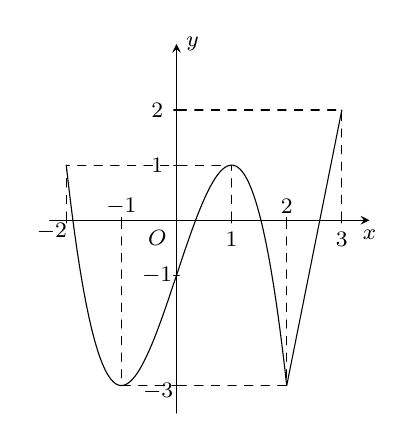
\begin{tikzpicture}[line join = round, line cap = round,font=\footnotesize,>=stealth,scale=.7] 
			\draw[->](-2.3,0)--(3.5,0)node[below]{$x$};
			\draw[->](0,-3.5)--(0,3.2)node[right]{$y$};
			\draw (0,0)node[below left]{$O$};
			\def\a{-1};
			\def\b{0};
			\def\c{3};
			\def\d{-1};
			\def\f(#1){\a*(#1)^3+\b*(#1)^2+\c*(#1)+\d};
			\draw[domain=-2:2,samples=100,smooth]plot(\x,{\f(\x)});
			\draw[dashed] (-2,0)--(-2,1)--(0,1) (1,0)--(1,1)--(0,1) (2,0)--(2,-3)--(0,-3) (-1,0)--(-1,-3)--(0,-3) (3,0)--(3,2)--(0,2);
			\draw (2,-3)--(3,2);
			\foreach \x/\g in {-2/-150,-1/90,1/-90,2/90,3/-90}\draw (\x,.05)--(\x,-.05)+(\g:.3)node{$\x$};
			\foreach \x/\g in {-3/-160,-1/180,1/180,2/180}\draw (.05,\x)--(-0.05,\x)+(\g:.3)node{$\x$};
		\end{tikzpicture}
	}
	\loigiai{
		Từ đồ thị hàm số, suy ra $\max\limits_{\left[-2;3\right]} f(x)=f(3)=2$
	}
\end{ex}

\begin{ex}%[2D1Y1-2]%[Dự án đề TT Toán NH25-26 Đợt 3- Nguyễn Thành Tiến]%[TT-SGD-Ninh Bình - Ninh BÌnh]%[GVPB: Phạm Văn Long]
	Cho hàm số $y=f(x)$ có bảng biến thiên như sau:
	\begin{center}
		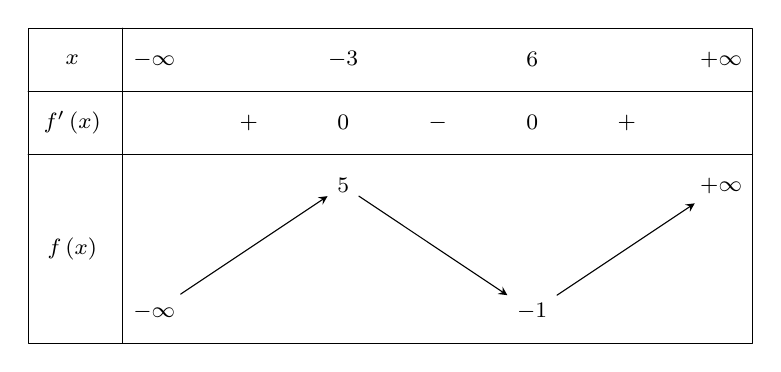
\begin{tikzpicture}[line join = round, line cap = round,font=\footnotesize,>=stealth,scale=.8]
			\foreach \x/\g in{-.3/x,1/-\infty,4/-3,7/6,10/+\infty}\path(\x,0)node{$\g$};
			\foreach \x/\g in {-.3/f'\left(x\right),2.5/+,4/0,5.5/-,7/0,8.5/+}\path(\x,-1)node{$\g$};
			\foreach \x/\y/\g in {-.3/-3/f\left(x\right),1/-4/-\infty,4/-2/5,7/-4/-1,10/-2/+\infty}\path(\x,\y)node(\x){$\g$};
			\foreach \x/\y in {1/4,4/7,7/10}\draw[-stealth] (\x)--(\y);
			\draw
			(-1,.5) rectangle (10.5,-4.5)
			(-1,-.5)--(10.5,-.5)
			(-1,-1.5)--(10.5,-1.5)
			(.5,.5)--(.5,-4.5);
		\end{tikzpicture}
	\end{center}
	Hàm số đã cho đồng biến trên khoảng nào sau đây?
	\choice
	 {$(-3;6)$}
	{\True $(6;+\infty)$}
	{$(-1;+\infty)$}
	{$(-\infty;5)$}
	\loigiai{
		Từ bảng biến thiên suy ra hàm số đồng biến trên các khoảng $(-\infty;-3)$ và $(6;+\infty)$. 
	}
\end{ex}

\begin{ex}%[2D3B2-1]%[Dự án đề TT Toán NH25-26 Đợt 3- Nguyễn Thành Tiến]%[TT-SGD-Ninh Bình - Ninh BÌnh]%[GVPB: Phạm Văn Long]
	Cho hàm số bậc hai $f(x)$. Biết đồ thị hàm số $y=f(x)$ cắt đường thẳng $y=9 x+8$ tại hai điểm $A$, $B$ phân biệt có hoành độ lần lượt là $x_A=-1$, $x_B=4$. Tính $I=\displaystyle\int\limits_{-1}^4 f'(x) \mathrm{\,d}x$.
	\choice
	{$I=43$}
	{$I=30$}
	{\True $I=45$}
	{$I=5$}
	 \loigiai{
		Theo giả thiết, ta suy ra $f(4)=y(4)=44$ và $f(-1)=y(-1)=-1$.\\
		Do đó
		\begin{eqnarray*}
			\displaystyle\int\limits_{-1}^4 f'(x) \mathrm{\,d}x=f(x)\Big|_{-1}^{4}=f(4)-f(-1)=44-(-1)=45.
		\end{eqnarray*}
	} 
\end{ex}

\begin{ex}%[2D3Y2-1]%[Dự án đề TT Toán NH25-26 Đợt 3- Nguyễn Thành Tiến]%[TT-SGD-Ninh Bình - Ninh BÌnh]%[GVPB: Phạm Văn Long]
	Nếu $\displaystyle\int\limits_0^1 f(x) \mathrm{\,d}x=2$ và $\displaystyle\int\limits_1^3 f(x) \mathrm{\,d}x=8$ thì $\displaystyle\int\limits_0^3 f(x) \mathrm{\,d}x$ bằng
	\choice
	{$16$}
	{$4$}
	{\True $10$}
	{$6$}
	\loigiai{
		Ta có
		\begin{eqnarray*}
			\displaystyle\int\limits_0^3 f(x) \mathrm{\,d}x&=&\displaystyle\int\limits_0^1 f(x) \mathrm{\,d}x+\displaystyle\int\limits_1^3 f(x) \mathrm{\,d}x\\
			&=&2+8=10.
		\end{eqnarray*}
	}
\end{ex}

\begin{ex}%[2H3B1-1]%[Dự án đề TT Toán NH25-26 Đợt 3- Nguyễn Thành Tiến]%[TT-SGD-Ninh Bình - Ninh BÌnh]%[GVPB: Phạm Văn Long]
	\immini[thm]{
		Cho hình lập phương $ABCD.A'B'C'D'$ (xem hình bên). Vectơ $\overrightarrow{AB}$ bằng vectơ nào sau đây?
		\choice
		{$\overrightarrow{CD}$}
		{$\overrightarrow{BC}$}
		{$\overrightarrow{AA'}$}
		{\True $\overrightarrow{A'B'}$}
	}{
		\begin{tikzpicture}[line join = round, line cap = round,font=\footnotesize,>=stealth,scale=.6]
			\path
			(0:0) coordinate (A)
			(0:6) coordinate (D)
			(-150:3) coordinate (B)
			($(B)+(D)-(A)$) coordinate (C)
			(90:4) coordinate (A')
			($(A')+(B)$) coordinate (B')
			($(A')+(D)$) coordinate (D')
			($(A')+(C)$) coordinate (C');
			\draw (A')--(B')--(C')--(D')--cycle (D)--(D') (B')--(B)--(C)--(C') (C)--(D);
			\draw[dashed] (A)--(A') (A)--(B) (A)--(D);
			\foreach \x/\g in {A/140,B/-90,C/-90,D/30,A'/90,B'/160,C'/90,D'/90}\draw[fill=white] (\x) circle (.05)+(\g:.3)node{$\x$};
		\end{tikzpicture}
	}
	\loigiai{
		Từ hình vẽ, suy ra
		\begin{eqnarray*}
			\vec{AB}=\vec{A'B'}.
		\end{eqnarray*}
	}
\end{ex}

\begin{ex}%[2D3Y2-1]%[Dự án đề TT Toán NH25-26 Đợt 3- Nguyễn Thành Tiến]%[TT-SGD-Ninh Bình - Ninh BÌnh]%[GVPB: Phạm Văn Long]
	Khẳng định nào sau đây đúng?
	\choice
	{$\displaystyle\int\limits 6^x \mathrm{\,d}x=\dfrac{6^{x+1}}{x+1}+C$}
	{$\displaystyle\int\limits 6^x \mathrm{\,d}x=6^x \cdot \ln 6+C$}
	{$\displaystyle\int\limits 6^x \mathrm{\,d}x=6^x+C$}
	{\True $\displaystyle\int\limits 6^x \mathrm{\,d}x=\dfrac{6^x}{\ln 6}+C$}
	\loigiai{
		Theo định nghĩa, ta có $\displaystyle\int\limits 6^x \mathrm{\,d}x=\dfrac{6^x}{\ln 6}+C$.
	}
\end{ex}


%%%%%-----Câu 7-----%%%%%
\begin{ex}%[2D4N1-1]%[Dự án đề TT Toán NH25-26 Đợt 3- Phan Trung Hiếu]%[TT-SGD-Ninh Bình - Ninh BÌnh]%[GVPB: Phạm Văn Long]
	Biết $\displaystyle\int f(x)\,\mathrm{d}x=x^2+\cos x+C$, khẳng định nào sau đây đúng?
	\choice
	{\True $f(x)=2x-\sin x$}
	{$f(x)=2x+\sin x$}
	{$f(x)=\dfrac{x^3}{3}+\sin x+C$}
	{$f(x)=\dfrac{x^3}{3}-\sin x+C$}
	\loigiai{
		Ta có $f(x)=2x-\sin x$.
	}
\end{ex}
%%%%%-----Câu 8-----%%%%%
\begin{ex}%[2H2N2-1]%[Dự án đề TT Toán NH25-26 Đợt 3- Phan Trung Hiếu]%[TT-SGD-Ninh Bình - Ninh BÌnh]%[GVPB: Phạm Văn Long]
	Trong không gian với hệ tọa độ $Oxyz$, cho véctơ $\vv{u}=(2;-1;3)$. Tìm tọa độ véctơ $3\vv{u}$.
	\choice
	{$3\vv{u}=(6;-1;3)$}
	{$3\vv{u}=(5;-3;6)$}
	{$3\vv{u}=(2;-1;9)$}
	{\True $3\vv{u}=(6;-3;9)$}
	\loigiai{
		Ta có $3\vv{u}=(6;-3;9)$.
	}
\end{ex}%%%%%-----Câu 9-----%%%%%
\begin{ex}%[2D3N1-2]%[Dự án đề TT Toán NH25-26 Đợt 3- Phan Trung Hiếu]%[TT-SGD-Ninh Bình - Ninh BÌnh]%[GVPB: Phạm Văn Long]
	Bảng sau đây biểu diễn mẫu số liệu ghép nhóm về cân nặng (đơn vị: kilôgam) của $40$ học sinh lớp $10A$ trong một trường trung học phổ thông.
	\begin{center}
		\begin{tabular}{|c|c|c|c|c|}
			\hline
			Nhóm&$[30;40)$&$[40;50)$&$[50;60)$&$[60;70)$\\
			\hline
			Tần số&$2$&$14$&$16$&$8$\\
			\hline
		\end{tabular}
	\end{center}
	Khoảng biến thiên của mẫu số liệu ghép nhóm trên bằng
	\choice
	{\True $40$}
	{$10$}
	{$30$}
	{$70$}
	\loigiai{
		Khoảng biến thiên của mẫu số liệu ghép nhóm trên bằng $70-30=40$.
	}
\end{ex}%%%%%-----Câu 10-----%%%%%
\begin{ex}%[2D1N5-1]%[Dự án đề TT Toán NH25-26 Đợt 3- Phan Trung Hiếu]%[TT-SGD-Ninh Bình - Ninh BÌnh]%[GVPB: Phạm Văn Long]
	\immini[thm]{
		Đường cong trong hình bên là đồ thị của hàm số nào sau đây?
		\choice
		{$y=\dfrac{2x+3}{x-1}$}
		{\True $y=\dfrac{x+1}{x-1}$}
		{$y=\dfrac{x-1}{x+1}$}
		{$y=\dfrac{x+1}{3x-3}$}
		\loigiai{
			Tiệm cận đứng của đồ thị hàm số là $x=1$.\\
			Tiệm cận ngang của đồ thị hàm số là $y=1$.\\
			Đường cong trong hình là đồ thị của hàm số $y=\dfrac{x+1}{x-1}$
		}
	}{
		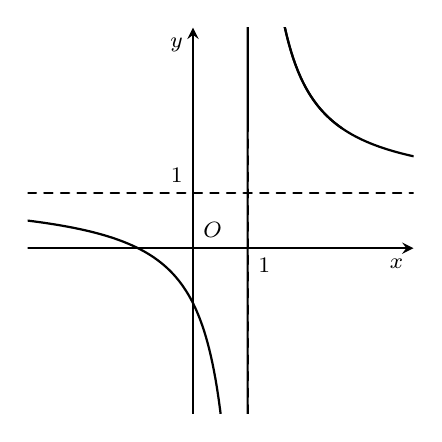
\begin{tikzpicture}[>=stealth, line cap=round, line join=round, font=\footnotesize, thick,scale=0.7]
			\def\xmin{-3}
			\def\xmax{4}
			\def\ymin{-3}
			\def\ymax{4}
			\clip (\xmin,\ymin) rectangle (\xmax,\ymax);
			\draw[->] (\xmin,0)--(0,0)node[above right]{$O$}--(\xmax,0)node[below left]{$x$};
			\draw[->] (0,\ymin)--(0,\ymax)node[below left]{$y$};
			\draw[dashed] (\xmin,1)--(0,1)node[above left]{$1$}--(\xmax,1);
			\draw[dashed] (1,\ymin)--(1,0)node[below right]{$1$}--(1,\ymax);
			\draw[samples=200, domain=1.3:\xmax] plot (\x, {(\x+1)/(\x -1)});
			\draw[samples=200, domain=\xmin:2.7] plot (\x, {(\x+1)/(\x -1)});
		\end{tikzpicture}
	}
\end{ex}%%%%%-----Câu 11-----%%%%%
\begin{ex}%[2H5N1-2]%[Dự án đề TT Toán NH25-26 Đợt 3- Phan Trung Hiếu]%[TT-SGD-Ninh Bình - Ninh BÌnh]%[GVPB: Phạm Văn Long]
	Trong không gian với hệ tọa độ $Oxyz$, cho mặt phẳng $(\alpha)\colon3x+2y-4z+1=0$. Véctơ nào sau đây là một véctơ pháp tuyến của mặt phẳng $(\alpha)$?
	\choice
	{$\vv{n_2}=(2;-4;1)$}
	{$\vv{n_4}=(-4;2;3)$}
	{\True $\vv{n_1}=(3;2;-4)$}
	{$\vv{n_3}=(3;-4;1)$}
	\loigiai{
		Một véctơ pháp tuyến của mặt phẳng $(\alpha)$ là $\vv{n_1}=(3;2;-4)$.
	}
\end{ex}
%%%%%-----Câu 12-----%%%%%
\begin{ex}%[2H5N1-1] %[Dự án đề TT Toán NH25-26 Đợt 3- Phan Trung Hiếu]%[TT-SGD-Ninh Bình - Ninh BÌnh]%[GVPB: Phạm Văn Long]
	Trong không gian với hệ tọa độ $Oxyz$, cho mặt phẳng $(\alpha)\colon x+y+z-4=0$. Điểm nào sau đây thuộc mặt phẳng $(\alpha)$?
	\choice
	{$N(2;3;0)$}
	{$P(4;1;1)$}
	{$Q(2;2;1)$}
	{\True $M(1;2;1)$}
	\loigiai{
		Ta có $1+2+1-4 = 0 $ nên điểm $M(1;2;1)$ thuộc mặt phẳng $(\alpha)$.
	}
\end{ex}

\TNTF
\begin{ex}%[2D4H1-3]%[Dự án đề TT Toán NH 2025-2026 Đợt 3-Lê Minh Thiện Anh]%[Sở GD Ninh Bình - Ninh Bình]%[GVPB: Phạm Văn Long]
	Cho hàm số $f(x) = \cos^2 \dfrac{x}{2}$.
	\choiceTF
	{$\displaystyle \int f(x)\mathrm{\,d}x = \dfrac{x}{2} - \dfrac{1}{2}\sin x + C$}
	{Nếu $F(x)$ là một nguyên hàm của hàm số $f(x)$ trên khoảng $(-\infty; +\infty)$ và thỏa mãn $F(0)=3$ thì $F\left(\dfrac{\pi}{6}\right) = \dfrac{\pi}{12} + \dfrac{11}{4}$}
	{\True $\displaystyle \int\limits_0^{\frac{\pi}{2}} f(x) \mathrm{\,d}x = a + b\pi$ ($a, b \in \mathbb{Q}$), trong đó $a^2 + b = \dfrac{1}{2}$}
	{\True Diện tích của hình phẳng giới hạn bởi đồ thị hàm số $y=f(x)$, $y=x^2-4+\cos^2 \dfrac{x}{2}$ và hai đường thẳng $x=0, x=3$ bằng $\dfrac{23}{3}$}
	\loigiai{
		Ta có $f(x) = \cos^2 \dfrac{x}{2} = \dfrac{1 + \cos x}{2} = \dfrac{1}{2} + \dfrac{1}{2}\cos x$.
		\begin{itemchoice}
			\itemch
			$\displaystyle \int f(x) \mathrm{\,d}x = \int \left(\dfrac{1}{2} + \dfrac{1}{2}\cos x\right) \mathrm{\,d}x = \dfrac{x}{2} + \dfrac{1}{2}\sin x + C$.			
			\itemch 
			Ta có $F(x) = \dfrac{x}{2} + \dfrac{1}{2}\sin x + C$. \\
			Vì $F(0)=3 \Rightarrow \dfrac{0}{2} + \dfrac{1}{2}\sin 0 + C = 3 \Rightarrow C = 3$. \\
			Khi đó $F\left(\dfrac{\pi}{6}\right) = \dfrac{\pi}{12} + \dfrac{1}{2}\sin\dfrac{\pi}{6} + 3 = \dfrac{\pi}{12} + \dfrac{13}{4}$.			
			\itemch 
			$\displaystyle \int\limits_0^{\frac{\pi}{2}} f(x) \mathrm{\,d}x = \left[ \dfrac{x}{2} + \dfrac{1}{2}\sin x \right]\bigg|_0^{\frac{\pi}{2}} = \left(\dfrac{\pi}{4} + \dfrac{1}{2}\right) - 0= \dfrac{1}{2} + \dfrac{1}{4}\pi$. \\
			Suy ra $a = \dfrac{1}{2}$, $b = \dfrac{1}{4}$. Vậy $a^2 + b = \left(\dfrac{1}{2}\right)^2 + \dfrac{1}{4} = \dfrac{1}{2}$.
			\itemch 
			Diện tích $S = \displaystyle \int\limits_0^3 |f(x) - (x^2 - 4 + f(x))|\mathrm{\,d}x = \int\limits_0^3 |4 - x^2|\mathrm{\,d}x$. \\
			$S = \displaystyle \int\limits_0^2 (4-x^2) \mathrm{\,d}x + \int\limits_2^3 (x^2-4) \mathrm{\,d}x = \dfrac{16}{3} + \dfrac{7}{3} = \dfrac{23}{3}$. 
		\end{itemchoice}
	}
\end{ex}

\begin{ex}%[2H2H2-4]%[Dự án đề TT Toán NH 2025-2026 Đợt 3-Lê Minh Thiện Anh]%[Sở GD Ninh Bình - Ninh Bình]%[GVPB: Phạm Văn Long]
	\immini[thm]{Cho hình hộp chữ nhật $ABCD.A'B'C'D'$ có đáy $ABCD$ là hình chữ nhật với $AB=5$, $AD=6$, $AA'=10$ và $G$ là trọng tâm của tam giác $BDA'$. Gắn một hệ tọa độ $Oxyz$ có gốc $O$ trùng với điểm $A$, tia $Ox$ trùng với tia $AB$, tia $Oy$ trùng với tia $AD$, tia $Oz$ trùng với tia $AA'$.
		\choiceTF
		{\True Tọa độ của điểm $C$ là $(5;6;0)$}
		{\True $|\vec{AC} + 2\vec{A'B}| = \sqrt{661}$}
		{Tọa độ điểm $G$ là $\left( 2; \dfrac{5}{3}; \dfrac{10}{3} \right)$}
		{\True $\vec{AG} \cdot \vec{B'C} = -\dfrac{64}{3}$}}
	{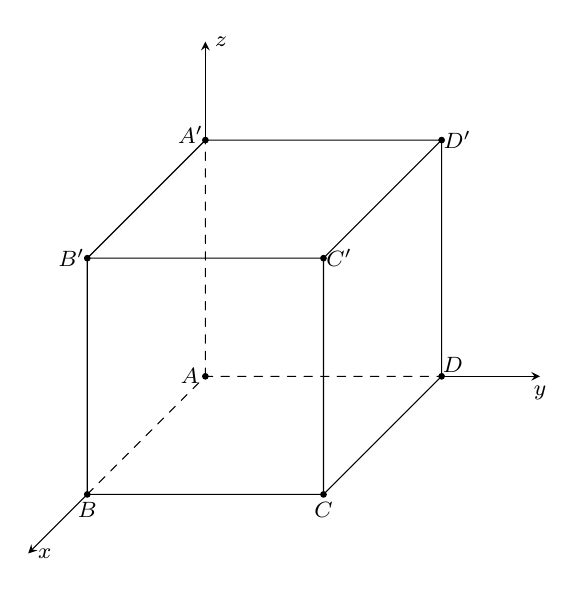
\begin{tikzpicture}[scale=1, font=\footnotesize, line join=round, line cap=round, >=stealth]
			\path
			(0,0) coordinate (B) 
			(3,0) coordinate (C) 
			(1.5,1.5) coordinate (A) 
			(A)+(3,0) coordinate (D);
			\foreach \x in {A,B,C,D}
			\path (\x)+(0,3) coordinate(\x');	
			\draw[dashed] (B)--(A)--(D) (A)--(A');
			\draw(B')--(C')--(D')--(A')--(B')--(B)--(C)--(D)--(D') (C)--(C');
			\draw[->](A')--(1.5,5.75)node[right]{$z$};
			\draw[->](D)--(5.75,1.5)node[below]{$y$};
			\draw[->](B)--(-0.75,-0.75)node[right]{$x$};
			\foreach \p/\g in {B/-90,C/-90,D/45,A/180,B'/180,C'/0,D'/0,A'/160}\draw[fill=black] (\p) circle (1pt)node[shift={(\g:.2)}]{$\p$};
		\end{tikzpicture}
	}
	\loigiai{
		Thiết lập tọa độ các điểm: $A(0;0;0)$, $B(5;0;0)$, $D(0;6;0)$, $C(5;6;0)$, $A'(0;0;10)$, $B'(5;0;10)$.
		\begin{itemchoice}
			\itemch Điểm $C$ có tọa độ $(5;6;0)$.			
			\itemch 
			$\vec{AC} = (5;6;0)$; $\vec{A'B} = (5;0;-10) \Rightarrow 2\vec{A'B} = (10;0;-20)$. \\
			$\vec{u} = \vec{AC} + 2\vec{A'B} = (15; 6; -20)$. \\
			$|\vec{u}| = \sqrt{15^2 + 6^2 + (-20)^2} = \sqrt{225 + 36 + 400} = \sqrt{661}$.
			\itemch 
			$G$ là trọng tâm $\triangle BDA'$\\
			$\Rightarrow x_G = \dfrac{5+0+0}{3} = \dfrac{5}{3}$; $y_G = \dfrac{0+6+0}{3} = 2$; $z_G = \dfrac{0+0+10}{3} = \dfrac{10}{3}$. \\
			Vậy $G\left( \dfrac{5}{3}; 2; \dfrac{10}{3} \right)$.
			\itemch 
			$\vec{AG} = \left( \dfrac{5}{3}; 2; \dfrac{10}{3} \right)$. \\
			$\vec{B'C} = (5-5; 6-0; 0-10) = (0; 6; -10)$. \\
			$\vec{AG} \cdot \vec{B'C} = \dfrac{5}{3} \cdot 0 + 2 \cdot 6 + \dfrac{10}{3} \cdot (-10) = -\dfrac{64}{3}$.
		\end{itemchoice}
	}
\end{ex}


\begin{ex}%[2D1V2-1]%[Dự án đề TT Toán NH25-26-Dot 3-Hồ Hải]%[SGD Ninh Bình - Tỉnh Ninh Bình][GVPB - GV Phạm Văn Long]
	Cho hàm số $f(x) = \mathrm{e}^{x^3-3x^2-9x+2026}$.	
	\choiceTF
	{Hàm số đã cho có đạo hàm là $f^\prime(x) = \mathrm{e}^{x^3-3x^2-9x+2026}$}
	{Hàm số $f(x)$ đồng biến trên khoảng $(-\infty;+\infty)$}
	{Hàm số $f(x)$ có hai cực trị trái dấu}
	{\True Tích giá trị lớn nhất và giá trị nhỏ nhất của hàm số $f(x)$ trên đoạn $\left[-2;2\right]$ bằng $\mathrm{e}^{4035}$}
	\loigiai{
		
		\begin{itemchoice}
			\itemch  Ta có $f^\prime(x) =  (3x^2-6x-9)\mathrm{e}^{x^3-3x^2-9x+2026}$.
			\itemch Xét $f^\prime(x) = 0\Leftrightarrow \hoac{&x= -1\\
				&x= 3.}$\newline
			Bảng biến thiên:
			\begin{center}
				
\begin{tikzpicture}
					\tkzTabInit[nocadre=false,lgt=1.2,espcl=2.5,deltacl=0.6]
					{$x$/0.6,$y'$/0.6,$y$/2}
					{$-\infty$,$-1$,$3$,$+\infty$}
					\tkzTabLine{,+,0,-,0,+,}
					\tkzTabVar
					{-/$0$,+/$\mathrm{e}^{2031}$,-/$\mathrm{e}^{1999}$,+/$+\infty$,}
				\end{tikzpicture}
			\end{center}
			
			\itemch Dựa vào bảng biến thiên, ta có $y_{\max}\cdot y_{\min} = \mathrm{e}^{4030} > 0$.
			\itemch Ta có $-1\in \left[-2;2\right] \Rightarrow \displaystyle\max\limits_{\left[-2;2\right]}f(x) = \mathrm{e}^{2031}$.\newline
			Lại có $f(-2) = \mathrm{e}^{2024}$ và $f(2) = \mathrm{e}^{2004}$.\newline
			Vậy $\displaystyle\max\limits_{\left[-2;2\right]}f(x)\cdot \displaystyle\min\limits_{\left[-2;2\right]}f(x) = \mathrm{e}^{2031}\cdot \mathrm{e}^{2004} = \mathrm{e}^{4035}$.
			
	\end{itemchoice}}
\end{ex}
\begin{ex}%[2H5V1-5]%[Dự án đề TT Toán NH25-26-Dot3-Hồ Hải]%[SGD Ninh Bình - Tỉnh Ninh Bình][GVPB - GV Phạm Văn Long]
	Trong không gian với hệ tọa độ $Oxyz$, cho ba điểm $A(-1;0;2)$, $B(2;2;1)$ và $C(0;-1;4)$.
	\choiceTF
	{Mặt phẳng $(Oxy)$ có phương trình là $x+y=0$}
	{Hình chiếu vuông góc của $B$ lên mặt phẳng $(Oxz)$ là điểm $B'(0;2;1)$}
	{\True Mặt phẳng đi qua $C$ và vuông góc với $AB$ có phương trình là $3x+2y-z+6=0$}
	{\True Gọi $(\alpha)$ là mặt phẳng chứa trục $Ox$ và song song với đường thẳng $AC$. Khoảng cách từ $B$ đến mặt phẳng $(\alpha)$ bằng $\sqrt{5}$}
	\loigiai{
		\begin{itemchoice}
			\itemch Phương trình mặt phẳng $(Oxy)\colon z=0$.
			\itemch Hình chiếu vuông góc của $B$ lên mặt phẳng $(Oxz)$ là $B^\prime (2;0;1)$.
			\itemch $\overrightarrow{AB} = (3;2;-1)$.\newline
			Mặt phẳng đi qua $C(0;-1;4)$ và có $\overrightarrow{AB} = (3;2;-1)$ là một vectơ pháp tuyến có phương trình tổng quát:
			\[3(x-0)+2(y+1)-1(z-4) = 0 \Leftrightarrow 3x+2y-z+6=0\]
			\itemch Vì mặt phẳng $(\alpha)$ chứa trục $Ox$ và song song với đường thẳng $AC$ nên có hai vectơ chỉ phương là $\overrightarrow{i} = (1;0;0)$ và $\overrightarrow{AC} =(1;-1;2)$.\newline
			Vectơ pháp tuyến: $\overrightarrow{n} = [\overrightarrow{i}, \overrightarrow{AC}] = (0;-2;-1)$.\newline
			Mặt phẳng $(\alpha)$ qua $O(0;0;0)$ và nhận $\overrightarrow{n} = (0;-2;-1)$ là một vectơ pháp tuyến có phương trình tổng quát:
			\[ -2y-z=0\Leftrightarrow 2y+z=0\]
			Khoảng cách từ điểm $B$ đến mặt phẳng $(\alpha)$ 
			$$\mathrm{d}(B,(\alpha)) = \dfrac{\left|0\cdot2 +2\cdot 2 +1\cdot 1 \right|}{\sqrt{0^2+2^2+1^2}} = \dfrac{5}{\sqrt{5}}=\sqrt{5}.$$
	\end{itemchoice}}
\end{ex}

\TNSA
\begin{ex}%[2H5V2-8]%[Dự án đề TT Toán NH25-26 đợt 3-Nguyễn Hoài Nam]%[SGD Ninh Bình-Ninh Bình]%[GVPB: Phạm Văn Long]
	Trong không gian với hệ tọa độ $Oxyz$ (đơn vị trên mỗi trục là km), một Radar phát hiện một chiếc máy bay di chuyển trên một đường thẳng với tốc độ và hướng bay không đổi. Máy bay bay từ điểm $A(712;200;6)$ đến điểm $B(802;220;8)$ trong $8$ phút và trong $4$ phút tiếp theo máy bay có vị trí là điểm $C(x;y;z)$. Giá trị $x+y+z$ bằng bao nhiêu?
	\shortans{$1\,086$}
	\loigiai{
		Ta có véc-tơ $\overrightarrow{AB}=(90;20;2)$. Đây là quãng đường máy bay đi được trong $8$ phút.\\
		Vì máy bay di chuyển trên một đường thẳng với tốc độ và hướng không đổi, nên trong $4$ phút tiếp theo, máy bay di chuyển một quãng đường tương ứng với véc-tơ $\overrightarrow{BC}$.\\
		Do thời gian $4$ phút bằng $\dfrac{1}{2}$ thời gian $8$ phút, ta có mối liên hệ giữa các véc-tơ dịch chuyển
		$$\overrightarrow{BC} = \dfrac{1}{2} \overrightarrow{AB} = \left(\dfrac{90}{2};\dfrac{20}{2};\dfrac{2}{2} \right) = (45;10;1).$$
		Tọa độ điểm $C$ được xác định bởi
		$\heva{&x=x_B+45=802+45=847\\ &y=y_B+10=220+10=230\ &z =z_B+1=8+1=9}  \Rightarrow C(847;230;9)$.\\
		Giá trị biểu thức cần tìm là $x+y+z=847+230+9=1 \,086$.
	}
\end{ex}

\begin{ex}%[2D4C3-2]%[Dự án đề TT Toán NH25-26 đợt 3-Nguyễn Hoài Nam]%[SGD Ninh Bình-Ninh Bình]%[GVPB: Phạm Văn Long]
	Trong hình bên là một chiếc đồng hồ treo tường cao cấp được thiết kế có phần ở giữa (phần tô đậm) dát vàng. Phần này được thiết kế như sau: 
	\begin{itemize}
		\item Vẽ hình lục giác đều $ABCDEF$ tâm $O$ và có cạnh bằng $4$ cm;
		\item Vẽ parabol $(C_1)$ tiếp xúc với các đường thẳng $OA$, $OB$ lần lượt tại $A$ và $B$;
		\item Tương tự vẽ parabol $(C_2)$ tiếp xúc với các đường thẳng $OB$, $OC$ lần lượt tại $B$ và $C$; parabol $(C_3)$ tiếp xúc với các đường thẳng $OC$, $OD$ lần lượt tại $C$ và $D$; \ldots; parabol $(C_6)$ tiếp xúc với các đường thẳng $OF$, $OA$ lần lượt tại $F$ và $A$.
	\end{itemize}
	Hình phẳng $(H)$ được giới hạn bởi sáu parabol $(C_1)$, $(C_2)$, $(C_3)$, $(C_4)$, $(C_5)$, $(C_6)$ (phần tô đậm) là phần sẽ được dát vàng. Hỏi phần dát vàng này có diện tích bằng bao nhiêu centimét vuông (không làm tròn kết quả các phép tính trung gian, chỉ làm tròn kết quả cuối cùng đến hàng phần chục)?
	\begin{center}
		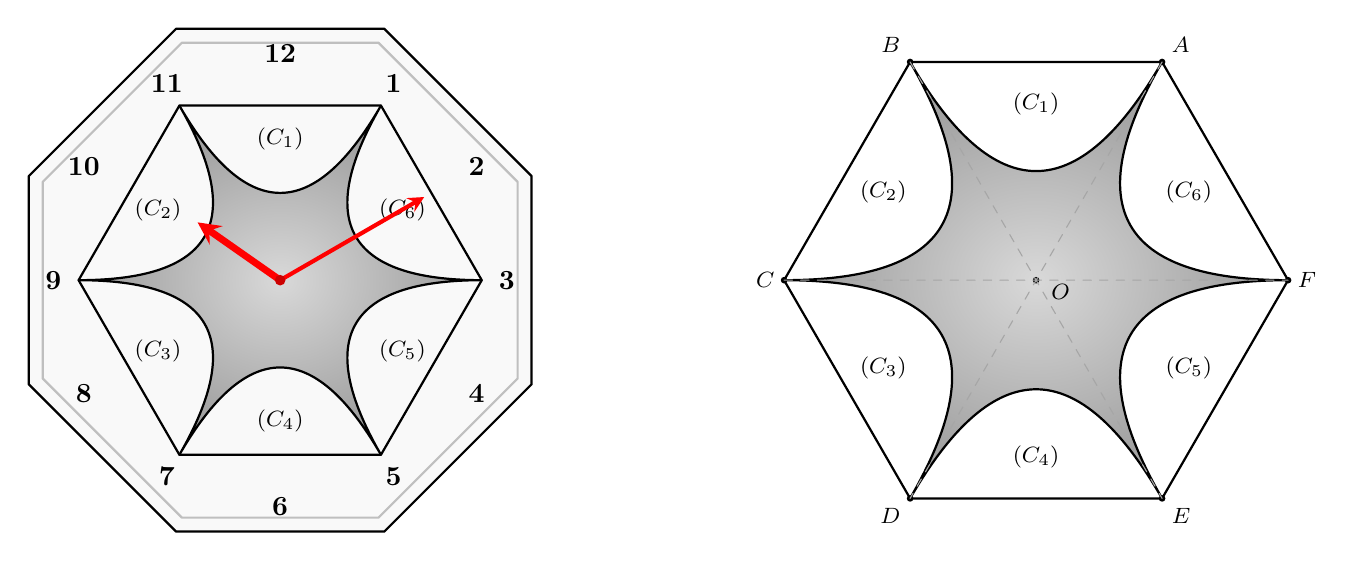
\begin{tikzpicture}[>=stealth, line join=round, line cap=round, font=\footnotesize, scale=0.8]
			
			% ==========================================
			% HÌNH 1: CHIẾC ĐỒNG HỒ THỰC TẾ (BÊN TRÁI)
			% ==========================================
			\begin{scope}[shift={(0,0)},scale=0.8]
				\coordinate (O) at (0,0);
				
				% 1. Vẽ viền bát giác đều bao bên ngoài (2 lớp)
				\draw[thick, fill=gray!5] 
				(22.5:5.4) -- (67.5:5.4) -- (112.5:5.4) -- (157.5:5.4) -- 
				(202.5:5.4) -- (247.5:5.4) -- (292.5:5.4) -- (337.5:5.4) -- cycle;
				\draw[thick, gray!50] 
				(22.5:5.1) -- (67.5:5.1) -- (112.5:5.1) -- (157.5:5.1) -- 
				(202.5:5.1) -- (247.5:5.1) -- (292.5:5.1) -- (337.5:5.1) -- cycle;
				
				% Tính toán tọa độ các đỉnh lục giác đều bên trong (R=4)
				\foreach \i/\a in {1/60, 2/120, 3/180, 4/240, 5/300, 6/360} {
					\coordinate (V\i) at (\a:4);
				}
				
				% Vẽ các đường chéo và cạnh lục giác
				\draw[thin, gray!70] (V1)--(V4) (V2)--(V5) (V3)--(V6);
				\draw[thick] (V1)--(V2)--(V3)--(V4)--(V5)--(V6)--cycle;
				
				% Tô màu và vẽ 6 parabol phần lõi
				\shade[inner color=gray!30, outer color=gray!80, draw=black, thick] 
				(V1) .. controls (60:1.333) and (120:1.333) .. (V2)
				.. controls (120:1.333) and (180:1.333) .. (V3)
				.. controls (180:1.333) and (240:1.333) .. (V4)
				.. controls (240:1.333) and (300:1.333) .. (V5)
				.. controls (300:1.333) and (360:1.333) .. (V6)
				.. controls (360:1.333) and (60:1.333) .. (V1);
				
				% Ký hiệu (C1), (C2)...
				\node at (90:2.8) {$(C_1)$};
				\node at (150:2.8) {$(C_2)$};
				\node at (210:2.8) {$(C_3)$};
				\node at (270:2.8) {$(C_4)$};
				\node at (330:2.8) {$(C_5)$};
				\node at (30:2.8) {$(C_6)$};
				
				% 2. Các cột số của đồng hồ (1 -> 12)
				\foreach \num/\angle in {1/60, 2/30, 3/0, 4/330, 5/300, 6/270, 7/240, 8/210, 9/180, 10/150, 11/120, 12/90} {
					\node[font=\bfseries\normalsize] at (\angle:4.5) {\num};
				}
				
				% 3. Kim đồng hồ (10 giờ 10 phút)
				% Kim phút chỉ ngay số 2 (góc 30 độ)
				\draw[->, red, line width=1.5pt] (0,0) -- (30:3.3); 
				% Kim giờ nhích qua số 10 một chút (10 giờ 10 phút -> góc 145 độ)
				\draw[->, red, line width=2.5pt] (0,0) -- (145:2.0);
				% Trục kim đồng hồ
				\fill[red!80!black] (0,0) circle (3pt);
			\end{scope}
			
			% ==========================================
			% HÌNH 2: MÔ HÌNH TOÁN HỌC GỐC (BÊN PHẢI)
			% ==========================================
			\begin{scope}[shift={(12,0)}] % Tịnh tiến sang phải 12 đơn vị để cách hình 1 tầm ~2cm
				\coordinate (O) at (0,0);
				
				% Tính toán tọa độ các đỉnh lục giác đều bán kính R=4
				\foreach \i/\a in {1/60, 2/120, 3/180, 4/240, 5/300, 6/360} {
					\coordinate (V\i) at (\a:4);
				}
				
				% Vẽ các đường chéo (sử dụng nét đứt - dashed) và cạnh lục giác
				
				\draw[thick] (V1)--(V2)--(V3)--(V4)--(V5)--(V6)--cycle;
				
				% Tô màu và vẽ 6 parabol bằng lệnh controls.
				\shade[inner color=gray!30, outer color=gray!80, draw=black, thick] 
				(V1) .. controls (60:1.333) and (120:1.333) .. (V2)
				.. controls (120:1.333) and (180:1.333) .. (V3)
				.. controls (180:1.333) and (240:1.333) .. (V4)
				.. controls (240:1.333) and (300:1.333) .. (V5)
				.. controls (300:1.333) and (360:1.333) .. (V6)
				.. controls (360:1.333) and (60:1.333) .. (V1);
				
				% Ký hiệu (C1), (C2)...
				\node at (90:2.8) {$(C_1)$};
				\node at (150:2.8) {$(C_2)$};
				\node at (210:2.8) {$(C_3)$};
				\node at (270:2.8) {$(C_4)$};
				\node at (330:2.8) {$(C_5)$};
				\node at (30:2.8) {$(C_6)$};
				
				% Tên các đỉnh
				\foreach \i/\n/\pos in {1/A/above right, 2/B/above left, 3/C/left, 4/D/below left, 5/E/below right, 6/F/right} {
					\fill (V\i) circle (1.5pt) node[\pos] {$\n$};
				}
				\fill (O) circle (1.5pt) node[below right, xshift=2pt, yshift=2pt] {$O$};
				\draw[dashed, thin, gray!70] (V1)--(V4) (V2)--(V5) (V3)--(V6);
			\end{scope}
		\end{tikzpicture}
	\end{center}
	\shortans{$13{,}9$}
	\loigiai{\immini[thm]{Chọn hệ trục tọa độ $Oxy$ sao cho gốc $O(0;0)$, tia $Ox$ trùng với tia $OF$, tia $Oy$ là tia phân giác của góc $\widehat{AOB}$ (tham khảo hình vẽ bên).\\
			Do $ABCDEF$ là lục giác đều cạnh bằng $4$ cm nên $OA=OB=OC=OD=OE=OF=4$ cm. Suy ra, $A=(4\cos 60^\circ;4\sin 60^\circ)=(2;2\sqrt{3})$ và\break $B=(4\cos 120^\circ;4\sin 120^\circ)=(-2;2\sqrt{3})$.\\
			Do prabol $(C_1)$ tiếp xúc với $OA$ và $OB$ nên parabol $(C_1)$ nhận $Oy$ làm trục đối xứng, do đó phương trình parabol $(C_1)$ có dạng $y=a x^2+b$. Suy ra, $y'=2a x$. \\
			Đường thẳng $OA$ có hệ số góc $k_A=\tan 60^\circ=\sqrt{3}$. Do $(C_1)$ tiếp xúc với $OA$ tại $A(2;2\sqrt{3})$ nên 
			$$y'(2)=k_A\Leftrightarrow 4a=\sqrt{3}\Leftrightarrow a=\dfrac{\sqrt{3}}{4}.$$
		}{\begin{tikzpicture}[scale=0.8, font=\footnotesize, line join=round, line cap=round, >=stealth]
				\coordinate (O) at (0,0);
				
				% Tính toán tọa độ các đỉnh lục giác đều bán kính R=4
				\foreach \i/\a in {1/60, 2/120, 3/180, 4/240, 5/300, 6/360} {
					\coordinate (V\i) at (\a:4);
				}
				
				% Vẽ các đường chéo (sử dụng nét đứt - dashed) và cạnh lục giác
				
				\draw[thick] (V1)--(V2)--(V3)--(V4)--(V5)--(V6)--cycle;
				
				% Tô màu và vẽ 6 parabol bằng lệnh controls.
				\shade[inner color=gray!30, outer color=gray!80, draw=black, thick] 
				(V1) .. controls (60:1.333) and (120:1.333) .. (V2)
				.. controls (120:1.333) and (180:1.333) .. (V3)
				.. controls (180:1.333) and (240:1.333) .. (V4)
				.. controls (240:1.333) and (300:1.333) .. (V5)
				.. controls (300:1.333) and (360:1.333) .. (V6)
				.. controls (360:1.333) and (60:1.333) .. (V1);
				
				% Ký hiệu (C1), (C2)...
				\node at (80:2.8) {$(C_1)$};
				\node at (150:2.8) {$(C_2)$};
				\node at (210:2.8) {$(C_3)$};
				\node at (260:2.8) {$(C_4)$};
				\node at (330:2.8) {$(C_5)$};
				\node at (30:2.8) {$(C_6)$};
				
				% Tên các đỉnh
				\foreach \i/\n/\pos in {1/A/above right, 2/B/above left, 3/C/above left, 4/D/below left, 5/E/below right, 6/F/above right} {
					\fill (V\i) circle (1.5pt) node[\pos] {$\n$};
				}
				\fill (O) circle (1.5pt) node[below right, xshift=2pt, yshift=2pt] {$O$};
				\draw[dashed, thin, gray!70] (V1)--(V4) (V2)--(V5) (V3)--(V6);
				\draw[-stealth] ($(O)!1.2!(V3)$)--($(O)!1.3!(V6)$) node [above] {$x$};
				\draw[-stealth] ($(O)!1.1!-90:(V6)$)--($(O)!1.2!90:(V6)$) node [right] {$y$};
		\end{tikzpicture}}
		Mặt khác, $A(2;2\sqrt{3})\in (C_1)$ nên $4a+b=2\sqrt{3}$, suy ra $b=2\sqrt{3}-4a=2\sqrt{3}-\sqrt{3}=\sqrt{3}$.\\
		Do đó, $(C_1)\colon y=\dfrac{\sqrt{3}}{4}x^2+\sqrt{3}$.\\
		Diện tích phần giới hạn bởi đường thẳng $AB$ và parabol $(C_1)$ là
		$$\mathrm{S}_1=\int\limits_{-2}^2 \left(2\sqrt{3}-\dfrac{\sqrt{3}}{4}x^2-\sqrt{3}\right)\mathrm{\,d}x=\int\limits_{-2}^2 \left(\sqrt{3}-\dfrac{\sqrt{3}}{4}x^2\right)\mathrm{\,d}x=\left.\left(\sqrt{3}x-\dfrac{\sqrt{3}}{12}x^3\right)\right|_{-2}^2=\dfrac{8\sqrt{3}}{3}.$$
		Suy ra, diện tích phần hình phẳng giới hạn bởi parabol $(C_1)$, $OA$ và $OB$ là 
		$$\mathrm{S}=\mathrm{S}_{OAB}-\mathrm{S}_1=\dfrac{4^2\sqrt{3}}{4}-\dfrac{8\sqrt{3}}{3}=\dfrac{4\sqrt{3}}{3}.$$
		Diện tích hình phẳng $(H)$ là
		$$\mathrm{S}_H=6\mathrm{S}=6\cdot\dfrac{4\sqrt{3}}{3}=8\sqrt{3}\approx 13{,}9.$$}
\end{ex}
%%=======Câu 3=======%%
\begin{ex}%[2H5V1-5]%[Dự án đề TT Toán NH25-26-Dot-3-Trung Kien]%[SGD Ninh Bình Lần 2 - Ninh Bình]%[GVPB-Phạm Văn Long]
	Trong không gian $Oxyz$ (đơn vị trên mỗi trục tọa độ là mét), một ngôi nhà (xem hình vẽ bên) có sàn nhà nằm ngang trên mặt phẳng $(\alpha) \colon y - z - 5 = 0$. Hai mái nhà (coi như là hai phần mặt phẳng) lần lượt nằm trên các mặt phẳng $(P) \colon 2x - 3y + z - 6 = 0$, $(Q) \colon 2x + y - 3z + 10 = 0$. Hỏi chiều cao của ngôi nhà tính từ nóc nhà (điểm cao nhất của mái nhà) đến sàn nhà là bao nhiêu mét (không làm tròn kết quả các phép tính trung gian, chỉ làm tròn kết quả cuối cùng đến hàng phần trăm)?
	\begin{center}
		\begin{tikzpicture}[scale=1, font=\footnotesize, line join=round, line cap=round, >=stealth, transform shape]
			\path 
			(-1.8,1.2) coordinate (C)
			(2.6,1.2) coordinate (E)
			(0.37,2.45) coordinate (D)
			(-1.2,2.4) coordinate (G)
			(0.37,3.26) coordinate (F)
			(2,2.4) coordinate (H)
			($(C)!0.15!(D)$) coordinate (A)
			($(E)!0.15!(D)$) coordinate (B)
			($(A)+(0,-2)$) coordinate (M)
			($(B)+(0,-2)$) coordinate (N)
			($(C)!0.65!(D)$) coordinate (A1)
			($(E)!0.65!(D)$) coordinate (B1)
			($(A1)!0.5!(B1)$) coordinate (O)
			($(M)!0.3!(N)$) coordinate (M1)
			($(M)!0.7!(N)$) coordinate (N1)
			;
			\draw (C)--(D)--(E) (G)--(F)--(H) (C)--(G) (E)--(H) (D)--(F)
			(A)--(B) (A)--(M) (B)--(N)--(M)
			;
			\draw(A1)--($(A1)+(0,-0.62)$) coordinate (A2) (B1)--($(B1)+(0,-0.62)$)coordinate (B2);
			\draw[pattern=dots] ($(O)+(0,-0.2)$) circle (8pt);
			\draw[pattern=horizontal lines] (A1)--(A)--(A2)--cycle;
			\draw[pattern=horizontal lines] (B1)--(B)--(B2)--cycle;
			\draw[pattern=horizontal lines] (M1)--($(M1)+(0,1.5)$)--($(N1)+(0,1.5)$)--(N1);
			
			\fill[gray!30] (A)--(B)--($(B)+(0,-0.1)$)--($(A)+(0,-0.1)$);
			\draw ($(A)+(0,-0.1)$)--($(B)+(0,-0.1)$);
			\draw (-1.8,0)coordinate(a)--(-3.5,-1.5)coordinate(b)--(1.5,-1.5)coordinate(c);
			\pic[draw,thin,angle radius=9mm,"$\alpha$"] {angle=c--b--a};
		\end{tikzpicture}
	\end{center}
	\shortans[oly]{$6{,}36$}
	\loigiai{
		Gọi $d$ là giao tuyến của hai mặt phẳng $(P)$ và $(Q)$. Khi đó $d \parallel (\alpha)$.\\
		Chọn điểm $M$ tùy ý thuộc $d$, tọa độ điểm $M$ là nghiệm của hệ phương trình
		$$\heva{&2x - 3y + z - 6 = 0\\&2x + y - 3z + 10 = 0.}$$
		Chọn $x=0$, ta được hệ $\heva{&- 3y + z - 6 = 0\\&y - 3z + 10 = 0} \Leftrightarrow \heva{&y=-1\\&z=3.}$\\
		Nên $M(0;-1;3)$.\\
		Chiều cao ngôi nhà tính từ nóc nhà bằng khoảng cách từ điểm $M$ đến mặt phẳng $(\alpha)$,
		$$\mathrm{d}(M,(\alpha))=\dfrac{|y_M-z_M-5|}{\sqrt{1^2+(-1)^2}}=\dfrac{9\sqrt{2}}{2} \approx 6{,}36.$$
		
	}
\end{ex}

%=======Câu 4=======%%
\begin{ex}%[2D1C3-6]%[Dự án đề TT Toán NH25-26-Dot-3-Trung Kien]%[SGD Ninh Bình Lần 2 - Ninh Bình]%[GVPB-Phạm Văn Long]
	Ông chủ của một ngôi nhà muốn làm một chiếc thang cứu hộ (coi như một đoạn thẳng) để sử dụng khi có nguy hiểm xảy ra. Khi chiếc thang được sử dụng thì một đầu của nó sẽ tiếp đất và một đầu còn lại sẽ đặt vào bức tường của ngôi nhà. Chiếc thang này được thiết kế để nó đứng dưới đất vươn qua hàng rào tựa vào ngôi nhà (tham khảo hình vẽ bên). Hàng rào cao $2{,}88$ mét được đặt song song và cách bức tường của ngôi nhà một khoảng bằng $1{,}8$ mét. Hỏi chiều dài ngắn nhất của chiếc thang bằng bao nhiêu mét (không làm tròn kết quả các phép tính trung gian, chỉ làm tròn kết quả cuối cùng đến hàng phần trăm)?
	\begin{center}
		\begin{tikzpicture}[scale=0.7, font=\footnotesize, line join=round, line cap=round, >=stealth, transform shape]
			\draw[fill=blue!30!white] (0,0)--(5,1)--(5,4)--(0,3)--cycle;
			\draw[fill=blue!30!black]
			(0,0)--(-3,1)--(-3,4)--(0,3)--cycle;			
			\draw (1.25,0.25)--++(0,3)
			(2.5,0.5)--++(0,3)
			(3.75,0.75)--++(0,3); 
			\draw[fill=yellow] (-0.53,2.89)--(5.53,4.11)--(2.01,5.63)--cycle;			
			\tikzset{hangrao/.pic={
					\draw[fill=gray] (0,0)--++(5/20,1/20)--++(0,2)--++(-5/40,1/20)--++(-5/40,-1/20)--cycle;
			}}
			\draw[fill=gray] (1,0)--(6,1)--++(0,-0.2)--++(-5,-1)--cycle;
			\foreach \x in {0,2,4,...,20}{\pic at (1+\x/4,-1+\x/20){hangrao};}		
			\draw[fill=yellow!70!black] (2.01,5.63)--(-0.53,2.89)--(-3.53,3.89)--(-0.66,6.52)--cycle;			
			\draw[line width=2pt] (2.5,2.99)--(4.26,-1)
			(2.98,3.09)--(4.74,-0.89)
			\foreach \x in {0.1,0.2,0.3,0.4,0.5,0.6,0.7,0.8,0.9}{
				($(2.5,2.99)!\x!(4.26,-1)$)--++(0.48,0.1)};
		\end{tikzpicture}
	\end{center}
	\shortans[oly]{}
	\loigiai{
		\begin{center}
			\begin{tikzpicture}[scale=1, font=\footnotesize, line join=round, line cap=round, >=stealth]
				\draw (0,0)--(4,0)--(0,3.84)--cycle
				(1.5,0)--(1.5,2.4);
				\fill 
				(0,0)node[below left]{$A$} circle (1pt)
				(4,0)node[below right]{$B$} circle (1pt)
				(0,3.84)node[above]{$C$} circle (1pt)
				(1.5,0)node[below]{$K$} circle (1pt)
				(1.5,2.4)node[above]{$H$} circle (1pt);
			\end{tikzpicture}
		\end{center}
		Minh hoạ bài toán như trên, với $B$ là vị trí đặt thang trên mặt đất, khoảng cách từ nhà đến hàng rào là $AK=1{,}8$ m và hàng rào có độ cao $HK=2{,}88$ m.\\
		Đặt $KB=x$, $x>0$ (m). Vì $HK \parallel AC$ nên $\dfrac{HK}{AC}=\dfrac{KB}{AB}$. Suy ra
		$$AC = AB \cdot \dfrac{HK}{KB} = (x+1{,}8) \cdot \dfrac{2{,}88}{x}.$$
		Xét tam giác $ABC$ vuông tại $A$, ta có
		$$BC^2= AC^2 + AB^2=\dfrac{2{,}88^2}{x^2}\cdot(x+1{,}8)^2 + (x+1{,}8)^2.$$
		Đặt $a=1{,}8$ và $b=2{,}88$, ta được
		\begin{eqnarray*}
			BC^2	&=& \dfrac{b^2}{x^2}\cdot(x+a)^2 + (x+a)^2\\
			&=& x^2 + \dfrac{2ab^2}{x} + 2ax + \dfrac{a^2b^2}{x^2} + a^2 + b^2\\
			&=& \left(x^2 + \dfrac{ab^2}{x} + \dfrac{ab^2}{x}\right) + \left(ax + ax + \dfrac{a^2b^2}{x^2}\right)+a^2+b^2\\
			&\ge& 3\sqrt[3]{a^2b^4}	+ 3\sqrt[3]{a^4b^2}	+a^2+b^2\\
			&\approx& 43{,}02.
		\end{eqnarray*}
		Dấu ``='' xảy ra khi $x^3=ab^2$.\\
		Vậy $BC$ nhỏ nhất bằng $\sqrt{43{,}02}\approx6{,}56$.}
\end{ex}
\begin{ex}%[2D3K3-3]%[Dự án đề TT Toán NH25-26 Đợt 3-Đỗ Chí Tâm]%[SGD Ninh Bình-Ninh Bình]%[GVPB:Phạm Văn Long]
	Có một hình phẳng $(H)$ (phần tô đậm trong hình vẽ bên) được tạo ra bằng cách vẽ một hình vuông có cạnh bằng $4$. Sau đó, ở bốn góc hình vuông đó vẽ bốn đường cong đều có tính chất là: tích khoảng cách từ một điểm bất kì thuộc mỗi đường cong đó đến hai trục đối xứng $d_1, d_2$ của hình vuông bằng $2$. Khi cho hình phẳng $(H)$ quay quanh trục $d_1$ ta sẽ thu được một vật thể tròn xoay, thể tích vật thể tròn xoay đó bằng bao nhiêu (không làm tròn kết quả các phép tính trung gian, chỉ làm tròn kết quả cuối cùng đến hàng phần chục)? 
	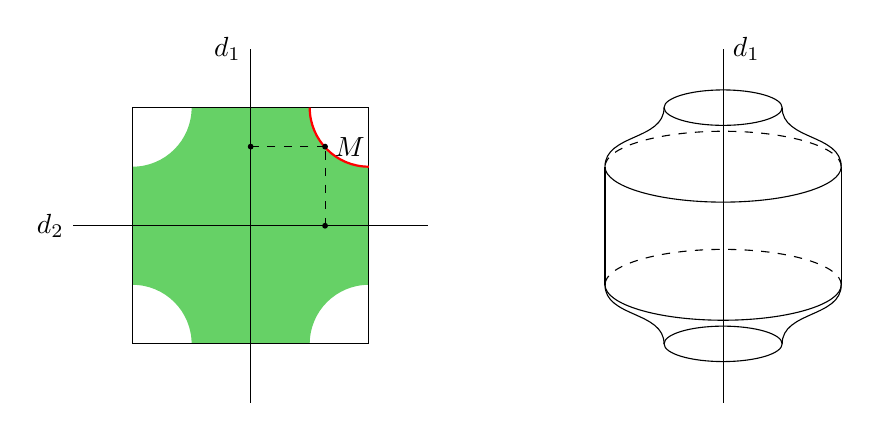
\begin{tikzpicture}[>=stealth, scale=1.5]
		
		% --- HÌNH 1: HÌNH PHẲNG ---
		\begin{scope}[xshift=0cm]
			% Tô màu xanh cho hình phẳng
			\fill[green!70!black!60] (0.5,1) -- (-0.5,1) 
			arc (0:-90:0.5) -- (-1,0.5) -- (-1,-0.5) 
			arc (90:0:0.5) -- (-0.5,-1) -- (0.5,-1) 
			arc (180:90:0.5) -- (1,-0.5) -- (1,0.5) 
			arc (270:180:0.5) -- cycle;
			
			% Vẽ khung hình vuông bao quanh
			\draw (-1,-1) rectangle (1,1);
			
			% Vẽ các trục đối xứng
			\draw (-1.5,0) -- (1.5,0) node[left] at (-1.5,0) {$d_2$};
			\draw (0,-1.5) -- (0,1.5) node[left] at (0,1.5) {$d_1$};
			
			% Chú thích "trục đối xứng"
			%			\node[right, scale=0.8] at (0,1.3) {truc doi xung};
			%			\node[right, scale=0.8] at (1,0.5) {truc doi xung};
			
			% Vẽ cung tròn màu đỏ và điểm M
			\draw[red, thick] (1,0.5) arc (270:180:0.5);
			%\fill (0.65, 0.86) circle (0.7pt) node[above right] {$M$};
			
			% Vẽ đường dóng từ M
			\draw[dashed] (0.63, 0.67) -- (0, 0.67);
			\draw[dashed] (0.63, 0.63) -- (0.63, 0);
			\fill (0, 0.67) circle (0.7pt);
			\fill (0.63, 0) circle (0.7pt);
			\fill (0.63, 0.67) circle (0.7pt) node[right]{$M$};
		\end{scope}
		
		% --- HÌNH 2: VẬT THỂ XOAY ---
		\begin{scope}[xshift=4cm]
			% Trục d1
			\draw (0,-1.5) -- (0,1.5) node[right] {$d_1$};
			
			% Các đường elip (mặt cắt ngang)
			\draw (0,1) ellipse (0.5 and 0.15); % Đỉnh trên
			\draw[dashed] (1,0.5) arc (0:180:1 and 0.3); % Giữa trên (phần khuất)
			\draw (1,0.5) arc (0:-180:1 and 0.3);        % Giữa trên (phần thấy)
			
			\draw[dashed] (1,-0.5) arc (0:180:1 and 0.3); % Giữa dưới (phần khuất)
			\draw (1,-0.5) arc (0:-180:1 and 0.3);        % Giữa dưới (phần thấy)
			
			\draw (0,-1) ellipse (0.5 and 0.15); % Đáy dưới
			
			% Vẽ các đường sinh bên ngoài
			\draw (-1, 0.5) -- (-1, -0.5); % Đường thẳng thân trụ trái
			\draw (1, 0.5) -- (1, -0.5);   % Đường thẳng thân trụ phải
			
			% Cung tròn tạo hình thắt (phần trên và dưới)
			\draw (-0.5, 1) to[out=270, in=90] (-1, 0.5);
			\draw (0.5, 1) to[out=270, in=90] (1, 0.5);
			\draw (-1, -0.5) to[out=270, in=90] (-0.5, -1);
			\draw (1, -0.5) to[out=270, in=90] (0.5, -1);
			
			% Đường trục đứt nét bên trong
			\draw[dashed] (0, 1) -- (0, -1);
		\end{scope}
		
	\end{tikzpicture}
	
	\shortans[oly]{$37{,}7$}
	\loigiai{
		\immini[thm]{
			Xét một phần đường cong ở cung phân từ thứ nhất trong hệ trục tọa độ $Oxy$ như hình.\\
			Vì $d(M, Ox)\cdot d(M,Oy)=2\Leftrightarrow y_M\cdot x_M=2$,\\
			nên $M\in (C): y=\dfrac{2}{x}$.\\
			$(C)$ giao với đường thẳng $y=2$ tai điểm $N(1; 2)$.\\
			Thể tích do $\dfrac{1}{4}$ hình $(H)$ (phần thuộc góc phần tư thứ nhất) quay quanh trục $Ox$ là\\
			$V_1=\displaystyle\pi\int_{0}^{1}2^2dx+\pi\int_{1}^{2}\dfrac{4}{x^2}dx=6\pi.$\\
			Vậy thể tích khối tròn xoay khi cho hình $(H)$ quay quanh trục $d_1$ là\\
			\hspace*{2cm}$V=2V_1=12\pi\approx 37{,}7$.
		}{
			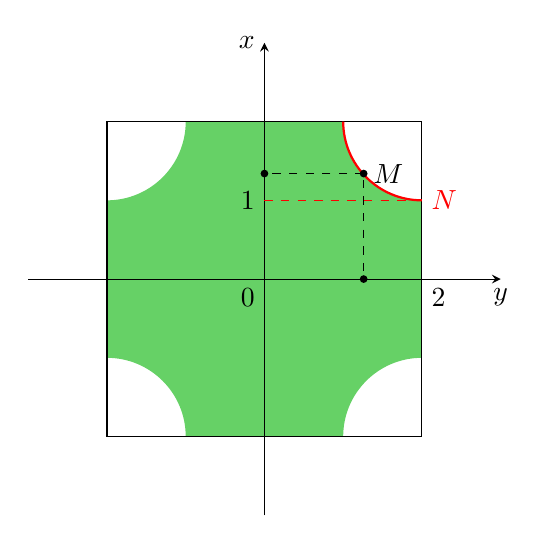
\begin{tikzpicture}[>=stealth, scale=2]
				
				% --- HÌNH 1: HÌNH PHẲNG ---
				\begin{scope}[xshift=0cm]
					% Tô màu xanh cho hình phẳng
					\fill[green!70!black!60] (0.5,1) -- (-0.5,1) 
					arc (0:-90:0.5) -- (-1,0.5) -- (-1,-0.5) 
					arc (90:0:0.5) -- (-0.5,-1) -- (0.5,-1) 
					arc (180:90:0.5) -- (1,-0.5) -- (1,0.5) 
					arc (270:180:0.5) -- cycle;
					
					% Vẽ khung hình vuông bao quanh
					\draw (-1,-1) rectangle (1,1);
					
					% Vẽ các trục đối xứng
					\draw[->] (-1.5,0) -- (1.5,0) node[below]{$y$};
					\draw[->] (0,-1.5) -- (0,1.5) node[left]{$x$};
					\draw[dashed, red](0,0.5)--(1,0.5) node[right]{$N$};
					
					% Chú thích "trục đối xứng"
					%			\node[right, scale=0.8] at (0,1.3) {truc doi xung};
					%			\node[right, scale=0.8] at (1,0.5) {truc doi xung};
					
					% Vẽ cung tròn màu đỏ và điểm M
					\draw[red, thick] (1,0.5) arc (270:180:0.5);
					%\fill (0.65, 0.86) circle (0.7pt) node[above right] {$M$};
					
					% Vẽ đường dóng từ M
					\draw[dashed] (0.63, 0.67) -- (0, 0.67);
					\draw[dashed] (0.63, 0.63) -- (0.63, 0);
					\fill (0, 0.67) circle (0.7pt);
					\fill (0.63, 0) circle (0.7pt);
					\fill (0.63, 0.67) circle (0.7pt) node[right]{$M$};
					\node[below right] at (1,0){$2$};
					\node[below left] at (0,0){$0$};
					\node[left] at(0,0.5){$1$};
				\end{scope}		
			\end{tikzpicture}
		}
	}
\end{ex}

\begin{ex}%[0D2V2-3]%[Dự án đề TT Toán NH25-26 Đợt 3-Đỗ Chí Tâm]%[SGD Ninh Bình-Ninh Bình]%[GVPB:Phạm Văn Long]
	Một công ty $A$ chuyên sản xuất giấy đã nhận được một đơn đặt hàng theo tháng từ đối tác $B$, mỗi tháng công ty $A$ phải cung cấp cho đối tác $B$ ít nhất $2800$ kg giấy in và $2400$kg giấy carton. Công ty $A$ sử dụng hai loại nguyên liệu là gỗ keo và gỗ bạch đàn. Từ một tấn gỗ keo sản xuất ra được $200$ kg giấy in và $300$ kg giấy carton; từ một tấn gỗ bạch đàn sản xuất ra được $300$ kg giấy in và $150$ kg giấy carton. Một tấn gỗ keo có giá là $1{,}2$ triệu đồng và một tấn gỗ bạch đàn có giá là $1{,}5$ triệu đồng. Biết mỗi tháng cơ sở cung cấp nguyên liệu chỉ cung cấp không quá $9$ tấn gỗ keo và không quá $10$ tấn gỗ bạch đàn. Số tiền nhỏ nhất mà công ty $A$ cần dùng mỗi tháng để mua nguyên liệu là bao nhiêu triệu đồng? 
	\shortans[oly]{$15$}
	\loigiai{
		\immini[thm]{
			Gọi $x$, $y$ lần lượt là số tấn gỗ keo và gỗ bạch đàn mà công ty $A$ cần dùng để sản xuất giấy cho đối tác $B$.\\
			Theo đề, ta có $\heva{&0\le x\le 9, 0\le y\le 10\\&200x+300y\ge 2800\\&300x+150y\ge 2400}\\$
			$\Leftrightarrow \heva{&0\le x\le 9, 0\le y\le 10\\&x+1{,}5y\ge 14\\&2x+y\ge 16}$\\
			$d_1: x+1{,}5y-14=0,\,\, d_2:2x+y-16=0$.\\
			$A(3;10), B(9;10), C\left(9;\dfrac{10}{3} \right), D(5;6).$\\
			Số tiền công ty $A$ dùng để mua nguyên vật liệu là\\
			$F(x;y)=1{,}2x+1{,}5y$ (triệu đồng).\\
			$F(A)=18{,}6, F(B)=25{,}8,$\\
			$ F(C)=15{,}8, F(D)=15$.\\
			Vậy số tiền thấp nhất mà công ty $A$ cần dùng để mua nguyên liệu mỗi tháng là $15$ (triệu đồng).
		}{
			\begin{tikzpicture}[scale=0.8, font=\footnotesize, line join=round, line cap=round, >=stealth]
				\draw[->] (-2,0)--(0,0)node[below left]{$O$}--(7.5,0)node[right]{$x$};
				\draw[->] (0,-2)--(0,8.2)node[right]{$y$};
				\clip (-2,-2) rectangle (7.6,8.2);
				\draw[red, thick] (-1,5.333)node[above]{$d_1$}--(7.5,-0.333);
				\draw[blue, thick] (0,8)--(5,-2); \node[right] at (4.7,-1.8) {$d_2$};
				\draw (-1,5)--(7,5) node[above]{$y=10$};
				\draw (4.5,-1)--(4.5,8) node[right]{$x=9$};
				\fill[pattern = north east lines, pattern color = black,opacity=0.45] (-1,5)--(7,5)--(7,9)--(-1,9)--cycle;%Tô nền
				\fill[pattern = north east lines, pattern color = blue,opacity=0.45] (4.5,-1)--(4.5,9)--(8,9)--(8,-1)--cycle;%Tô nền
				\fill[color =magenta!60,opacity=0.45] (-1,5.333)--(7.5,-0.333)--(7.5,-3)--(-1,-3)--cycle;%Tô nền
				\fill[color =gray!60,opacity=0.45] (0,8)--(-1,8)--(-1,-3)--(5,-2)--cycle;%Tô
				\fill[red] (4.5, 5) circle(2pt) node[below left]{$B$};
				\fill[red] (1.5, 5) circle(2pt) node[below right]{$A$};
				\fill[red] (4.5, 1.666) circle(2pt) node[above left]{$C$};
				\fill[red] (2.5, 3) circle(2pt) node[right]{$D$};
			\end{tikzpicture}
		}
	}
\end{ex}
\Closesolutionfile{ans}
% \inputansbox{6}{ans/ans-KSCL-NinhBinh-TLN}

>>>>>>> 33890a9ce1cfbd3079ed36a93e836cf3ef1fde30
